\chapter{Diverted Geometry}
\label{chap:TCV}

\begin{chaptersummarybox}
	The electromagnetic model is tested on a realistic X-point configuration based on the TCV-X21 benchmark case. In a flux-driven simulation with an injected power of 150kW, representative of an L-mode plasma, we compare the same four scenarios (electrostatic, electrostatic with electron inertia, magnetic induction, and magnetic induction with flutter). Overall, the plasma behavior is consistent with the findings in the limited geometries. Electron inertia does not significantly impact turbulence levels or mid-plane profiles. However, magnetic induction considerably increases cross-field particle and heat transport, leading to a strong flattening of density and temperature profiles, such that an energetic quasi-steady state is reached within 3ms of simulated plasma time. Flutter counteracts the inductive destabilization and restores steep profiles at a lower turbulence level than in the electrostatic cases. \\
	Numerically, electron inertia accelerates the simulation by improving the condition number of the vorticity equation. The increase in system size due to magnetic induction slightly deteriorates CPU time, even though the number of iterations required for convergence remains below the level of the electrostatic case. With flutter, code performance worsens considerably, mainly due to the radial connection between flux surfaces in the geometry, which adds coupling in the implicit viscosity, parallel heat conduction, and vorticity problems. \\
	In a preliminary study, the injected power was increased to 1.2MW with the full electromagnetic model and additional fluid neutrals. Under these conditions, flutter-induced radial heat transport in the parallel heat conduction starts to compete with energy transport by ExB drifts and eventually dominates the total electron power across the separatrix. Simultaneously, the fluctuating magnetic field shapes island-like patterns along the separatrix.
\end{chaptersummarybox}

\newpage


To demonstrate the abilities of SOLEDGE3X to perform electromagnetic turbulence simulations of a realistic tokamak geometry, the configuration of the test cases has been inspired by the TCV-X21 benchmark\cite{oliveira2022}. This latter addresses L-mode discharges in TCV with a single lower X-point. 


\section{Electrostatic versus electromagnetic scenarios}

The semi-implicit time discretization implemented in this model allows comparisons to be made between the electrostatic and electromagnetic models using the same code. Four cases have therefore been considered here: electrostatic (ES), electrostatic with electron inertia (ES-inert), electromagnetic (EM), and electromagnetic with flutter (EM-flutter).

\subsection{Simulation set-up}

The plasma is pure deuterium, and only a quarter-torus with a relatively low resolution of approximately 1.9 million cells has been considered to speed up computations (see the mesh in a poloidal plane in Fig. \ref{fig:TCVmesh}). A constant heat source of 25 kW is applied to both electrons and ions, equating to a full-torus equivalent total Ohmic heating of 200 kW. The external toroidal magnetic field is $B_t = 0.95$ T, and the density at the separatrix is targeted to $7 \cdot 10^{18}$ part/m$^3$. \newline

Since the aim of these preliminary computations was to focus on electromagnetic effects, neutrals have been omitted to speed up the convergence of the solutions. Simulations with a more complete physical model will be performed in a further work, including in particular the latest fluid neutral model \cite{quadri2024} developed for regimes dominated by charge exchanges \cite{horsten2017}. \newline

In all cases, the initial condition is the corresponding 2D transport solution obtained by increased perpendicular diffusion coefficients. \newline

In Fig. \ref{fig:EMsnapshots}, typical poloidal cuts of important plasma fields are shown. The local value of $\beta$ varies between $10^{-3}$ at the hot core boundary, $10^{-4}$ around the separatrix and divertor region, and $10^{-5}$ or lower in the far SOL. Consequently, the flutter perturbation $\tilde{B}$ of the magnetic field remains small compared to the equilibrium field, barely exceeding 0.1\% of $B_t$ on the hot core side of the domain. The advection velocity associated with the flutter is also minimal, contributing to less than 0.1\% of the cross-field transport, dominated by the electric "ExB" drift. \newline

\begin{figure}[H]\centering
	\centering
	\makebox[\textwidth][c]{\includegraphics[width=1.3\textwidth]{schemes/TCVnoNeutrSnapshots.png}}    
	\caption[Simulation snapshots of the full electromagnetic scenario with flutter]{Simulation snapshots of the full electromagnetic scenario with flutter. The first poloidal plane is shown after 6 ms simulated plasma time on the TCV case. From left to right, the first row shows the ion density $n_i$, the electron temperature $T_e$, the electric potential $\Phi$, and the radial "ExB" drift velocity $v_E^\psi$. The second row shows the parallel magnetic potential $A_\parallel$, the parallel current density $j_\parallel$, the amplitude of the flutter field $\norm{\mathbf{\tilde{B}}}$, and the radial flutter advection velocity $v_{\tilde{b}^\psi}$.}
	\label{fig:EMsnapshots}
\end{figure}



\subsection{Comparison between the scenarios}

We now compare the impact of the different levels of new physics on the TCV scenario. Since turbulent structures are essentially driven by the electric "ExB" drift, we consider the associated total kinetic energy $E_{ExB} = \frac{1}{2}m_i \int_V n_i \norm{v_E}^2 dV$ to estimate the turbulence level. As shown in Fig. \ref{fig:KE_ExB}, a finite electron mass does not change the energy level with respect to the reference electrostatic scenario. Next, adding magnetic induction with $A_\parallel$ further amplifies the turbulent interchange. This enhancement arises from the increased coupling between the magnetic and electric fields, leading to more instabilities and modified turbulent dynamics. Consequently, turbulent filaments give way to smaller, rounder blobs. Finally, the inclusion of flutter has a stabilizing effect on the turbulence, where fluctuations fall again to the level in the electrostatic case. Nonlinear effects in the parallel current equation, namely from the parallel pressure gradient $\nabla_\parallel p_e$, substantially impact the profiles of $j_\parallel$ and hence the response of the potential $\Phi$. The direct consequence is a modification of the radial electric field and a modified evolution of "ExB" drifts. This does not contradict our previous observation that magnetic advection is negligible with respect to the electric drift. \newline

With a different turbulence level, the heat exhaust is also affected, as shown in Fig. \ref{fig:HeatExhaust}. Without radiative effects, the quasi-totality of the heat leaves the tokamak at two divertor targets. The supplementary radial turbulent transport in the magnetic inductive scenario allows more hot particles to cross the separatrix from the core, which will then eventually reach the divertor. Overall, the heat flux is multiplied by a factor of 10. Electron inertia alone leads to an increase by a factor of 2, despite very similar turbulence levels. This phenomenon needs further investigation. Flutter does not reduce further the heat exhaust as one might expect because it is already very low in the electrostatic case. \newline

\begin{figure}[H]\centering
	\begin{subfigure}[t]{0.45\textwidth}
		\centering
		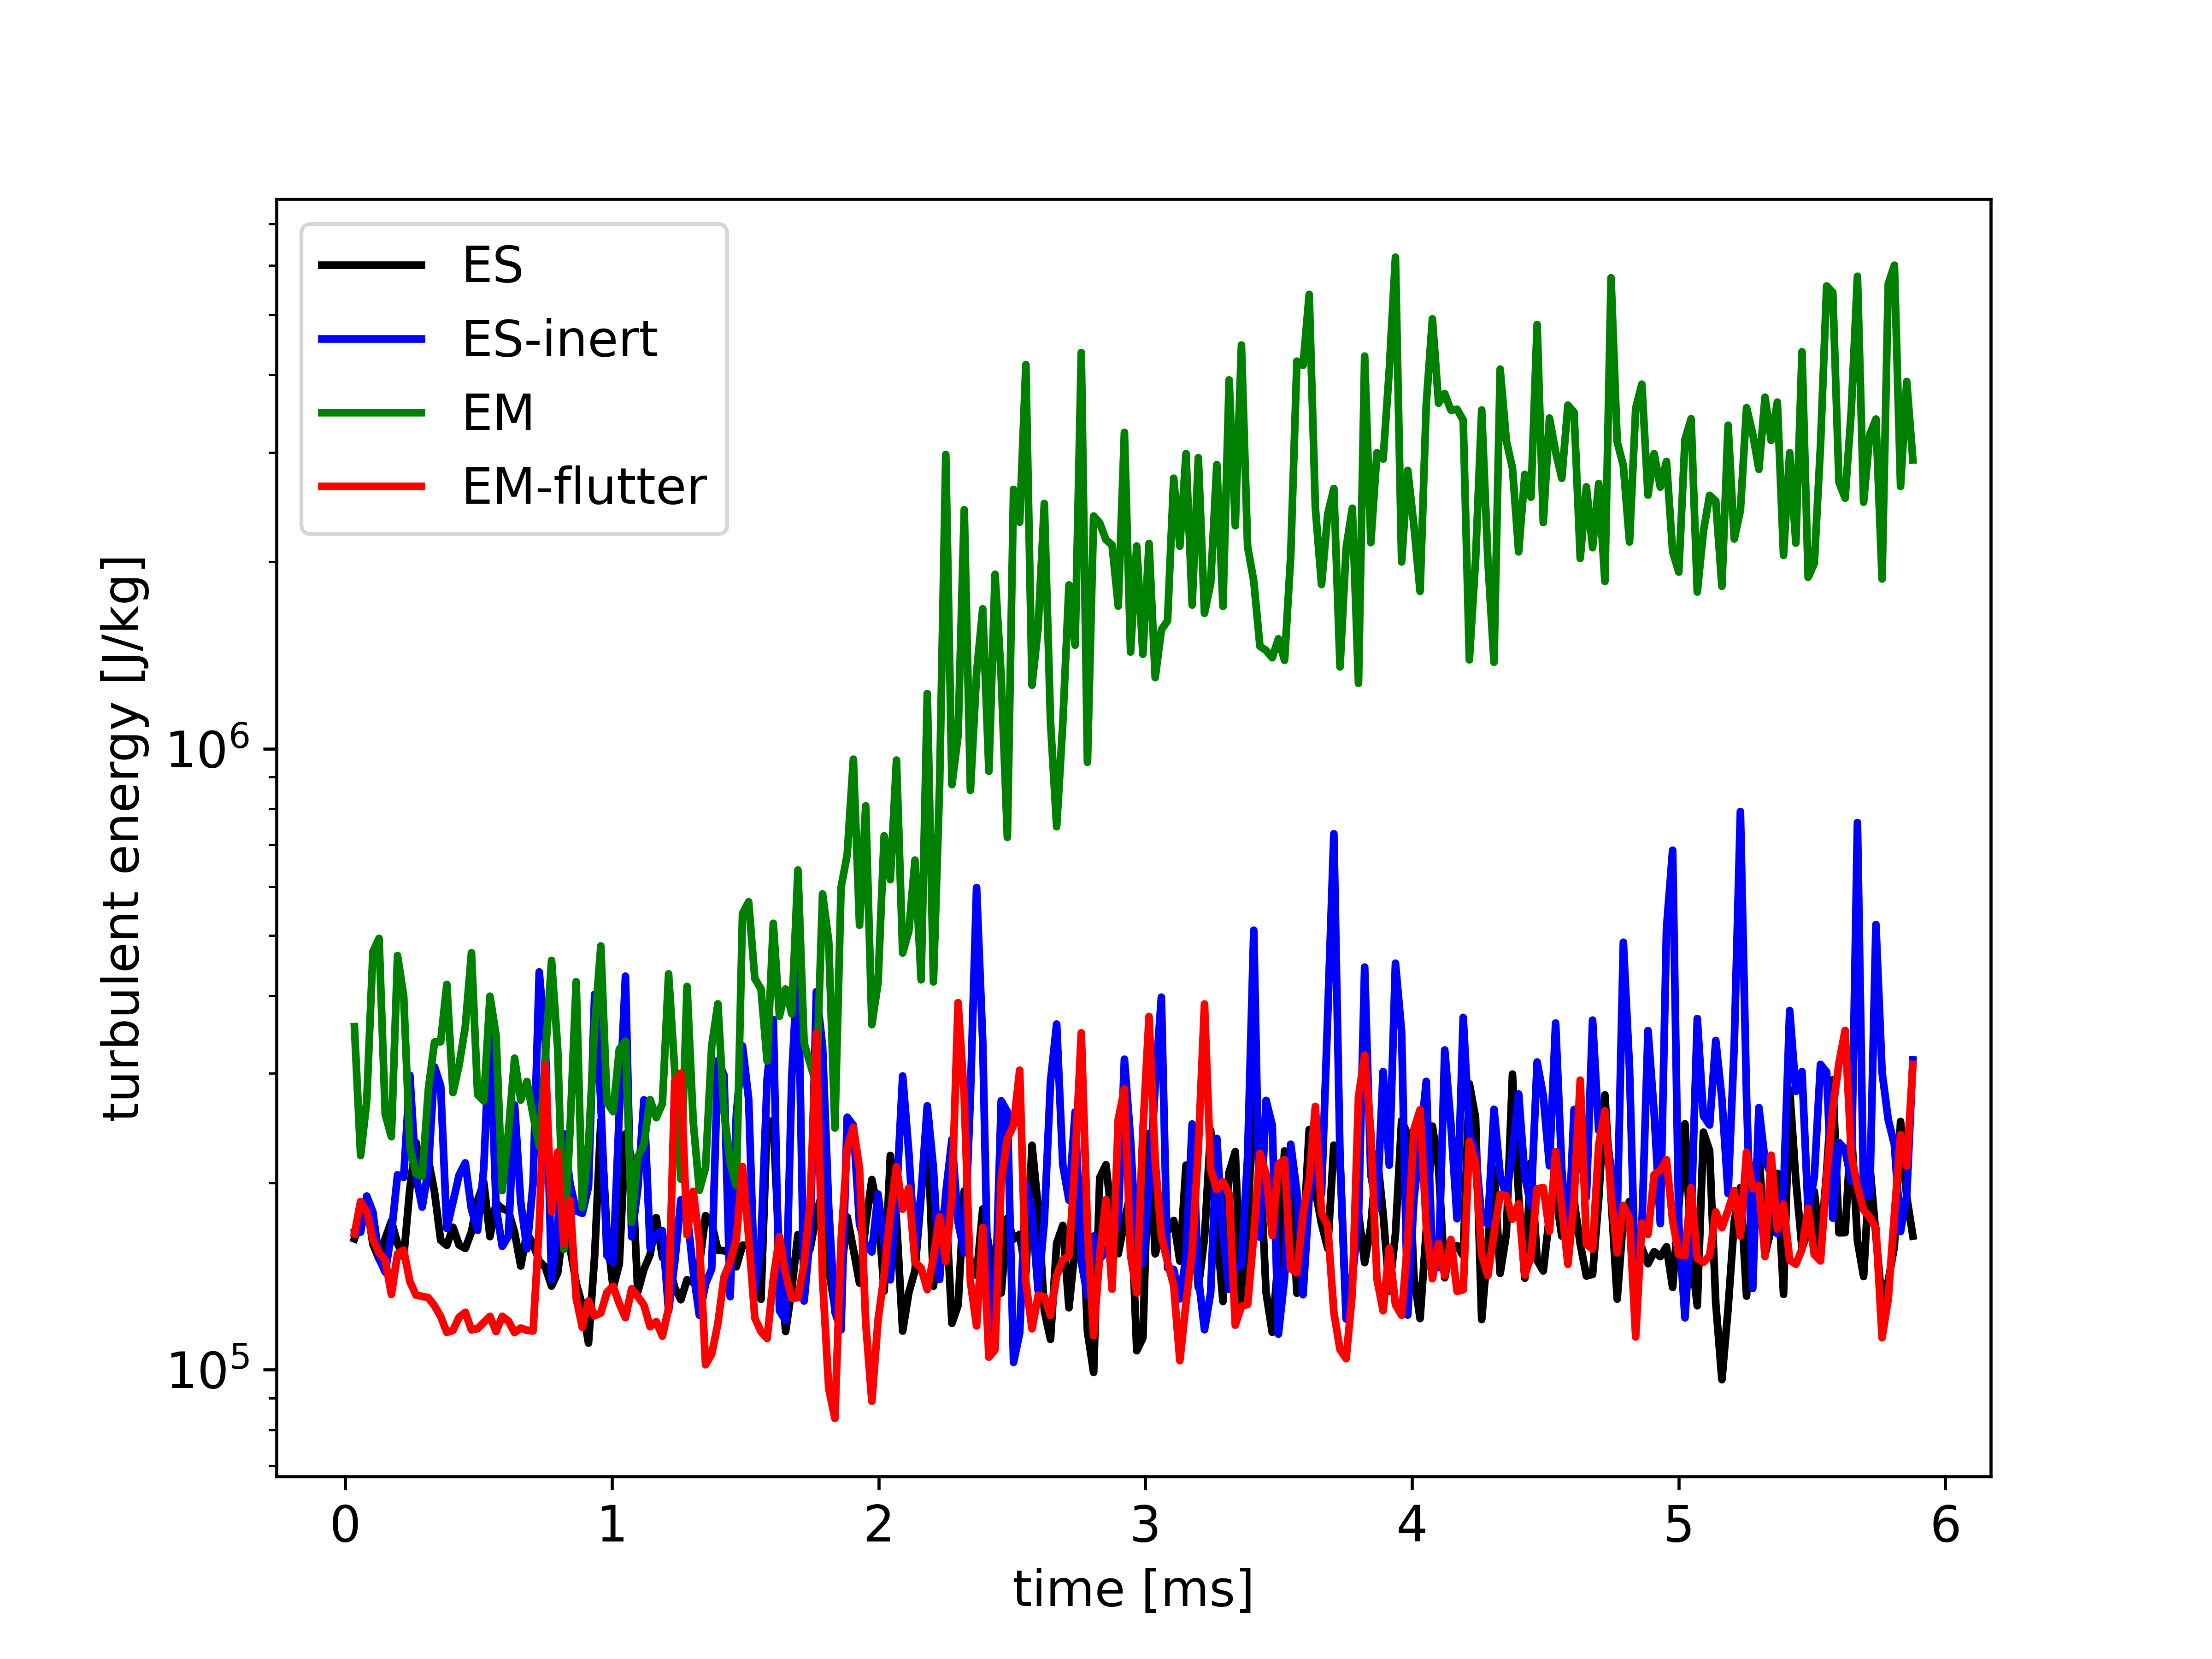
\includegraphics[width=1\textwidth]{schemes/Eturb_sep.png}
		\subcaption{Turbulent kinetic energy of D$^+$ ions \\ at the separatrix.}
		\label{fig:KE_ExB}
	\end{subfigure}
	\begin{subfigure}[t]{0.45\textwidth}
		\centering
		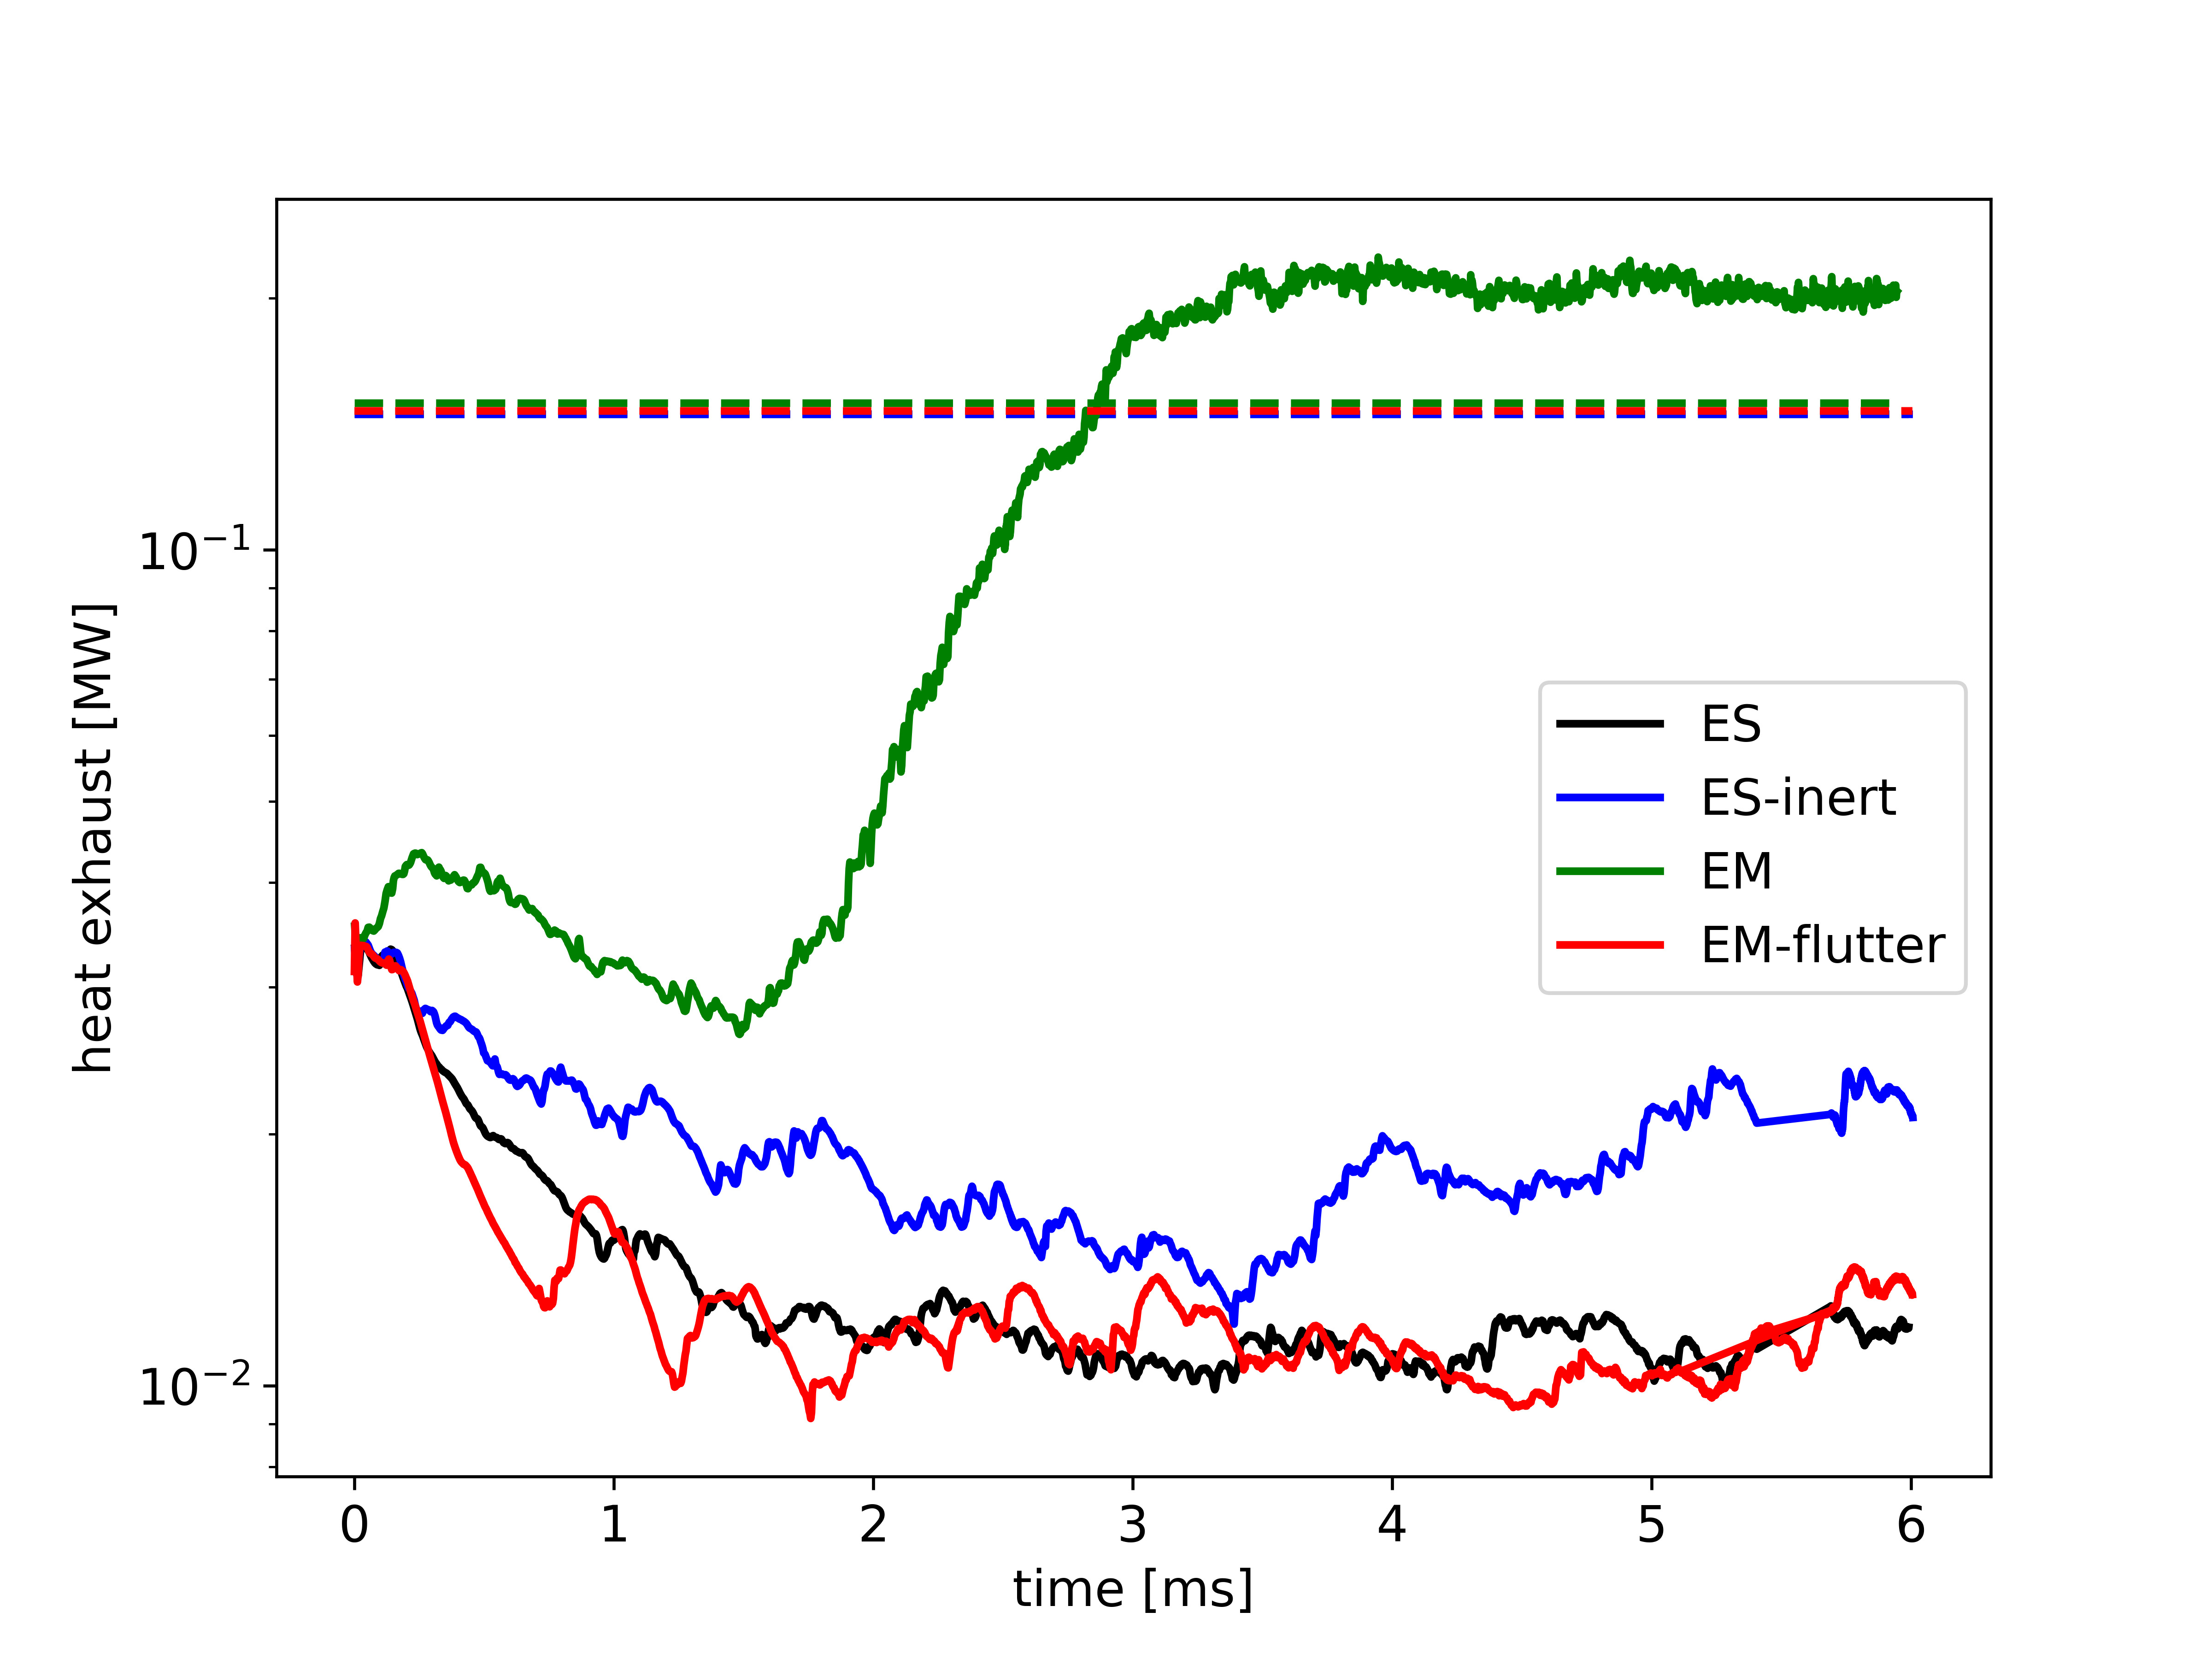
\includegraphics[width=1\textwidth]{schemes/heatExhaust_noNeutr.jpg}
		\subcaption{Total heat exhaust}
		\label{fig:HeatExhaust}
	\end{subfigure}
	\caption[Evolution of the turbulent energy and heat exhaust over time iterations on the turbulent TCV scenario]{Evolution of the turbulent energy and heat exhaust over time iterations on the turbulent TCV scenario. It indicates the turbulence level and its consequence on the total heat transport.}
	\label{fig:plasmaEvolution}
\end{figure}

The change in turbulence intensity naturally impacts the mean profiles in Fig. \ref{fig:OMP_profiles}. The most noticeable change affects the electromagnetic inductive scenario, where density and temperature gradients are considerably reduced by the additional radial turbulent transport. Again, the finite electron mass has no significant impact, and the reduced turbulence levels by flutter lead to steeper gradients. At this point, we stress the similarity to the simplified drift wave simulations on slab in Sec. \ref{ssec:plasmaturbslab}, where the gradients from the dense core follow the same pattern. \newline

\begin{figure}[H]\centering
	\begin{subfigure}[t]{0.30\textwidth}
		\centering
		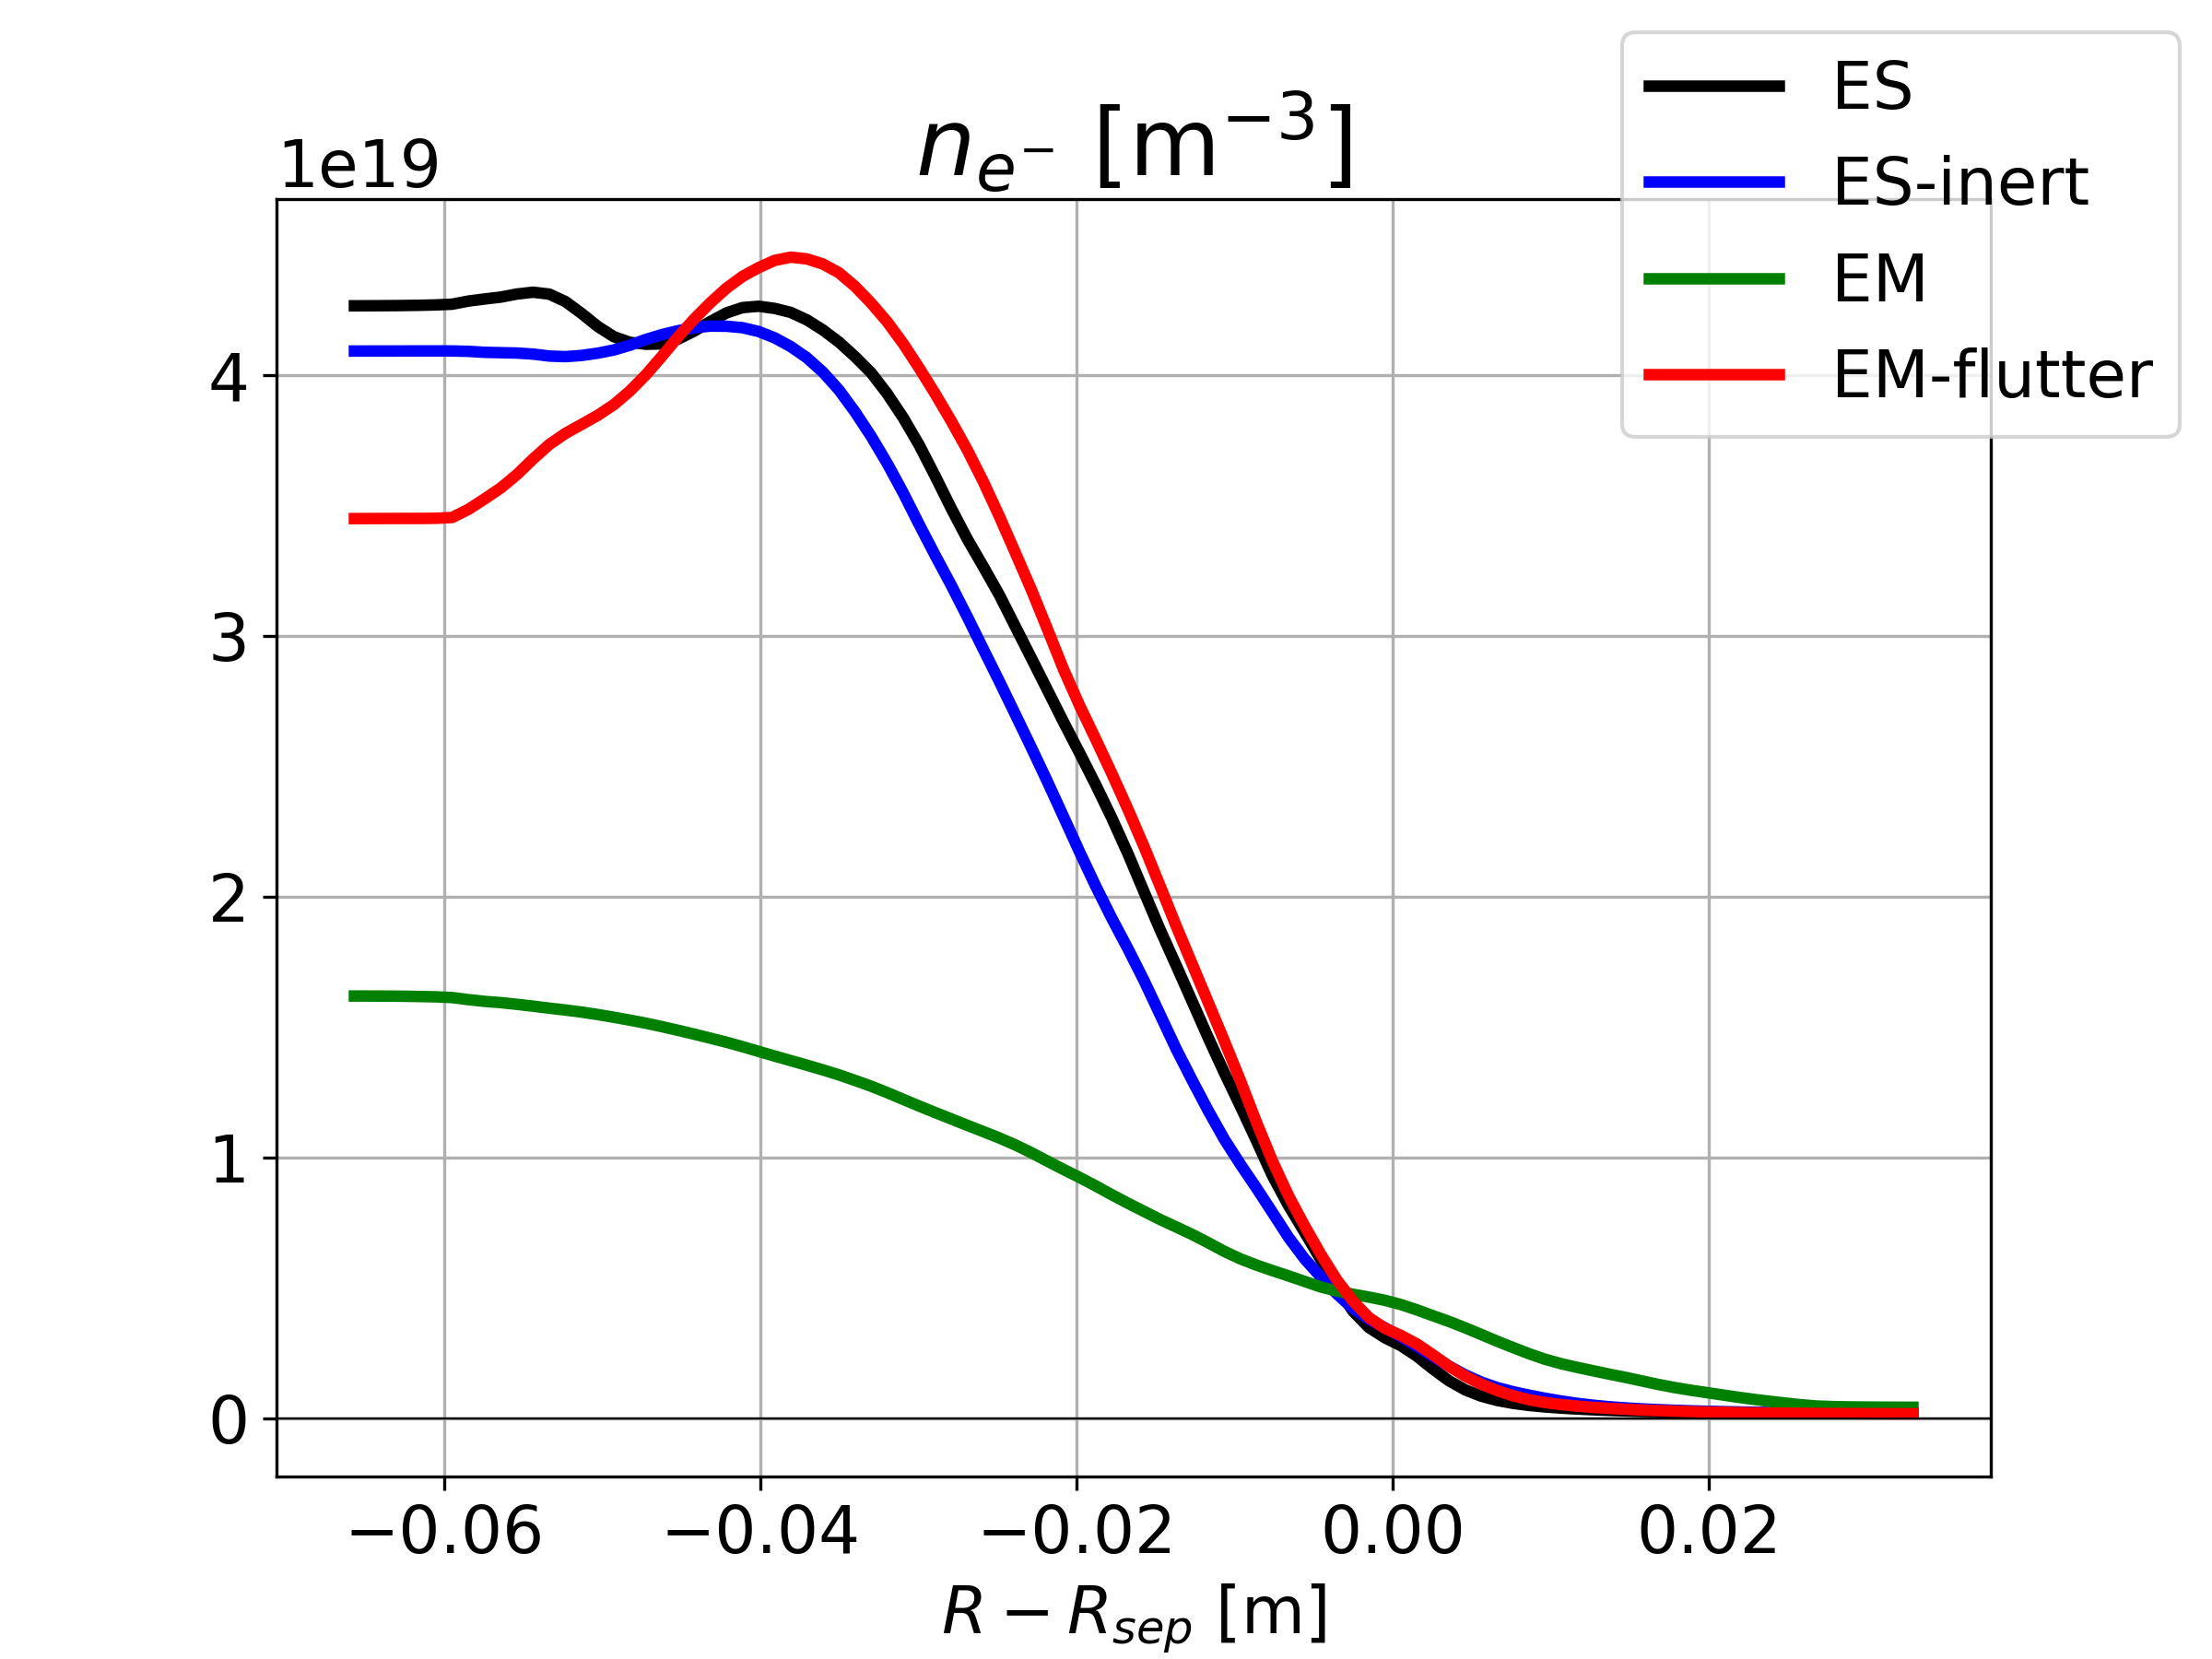
\includegraphics[width=1\textwidth]{schemes/OMP_profiles_e-_n.png}
		\subcaption{Plasma density $n$}
	\end{subfigure}	
	\begin{subfigure}[t]{0.30\textwidth}
		\centering
		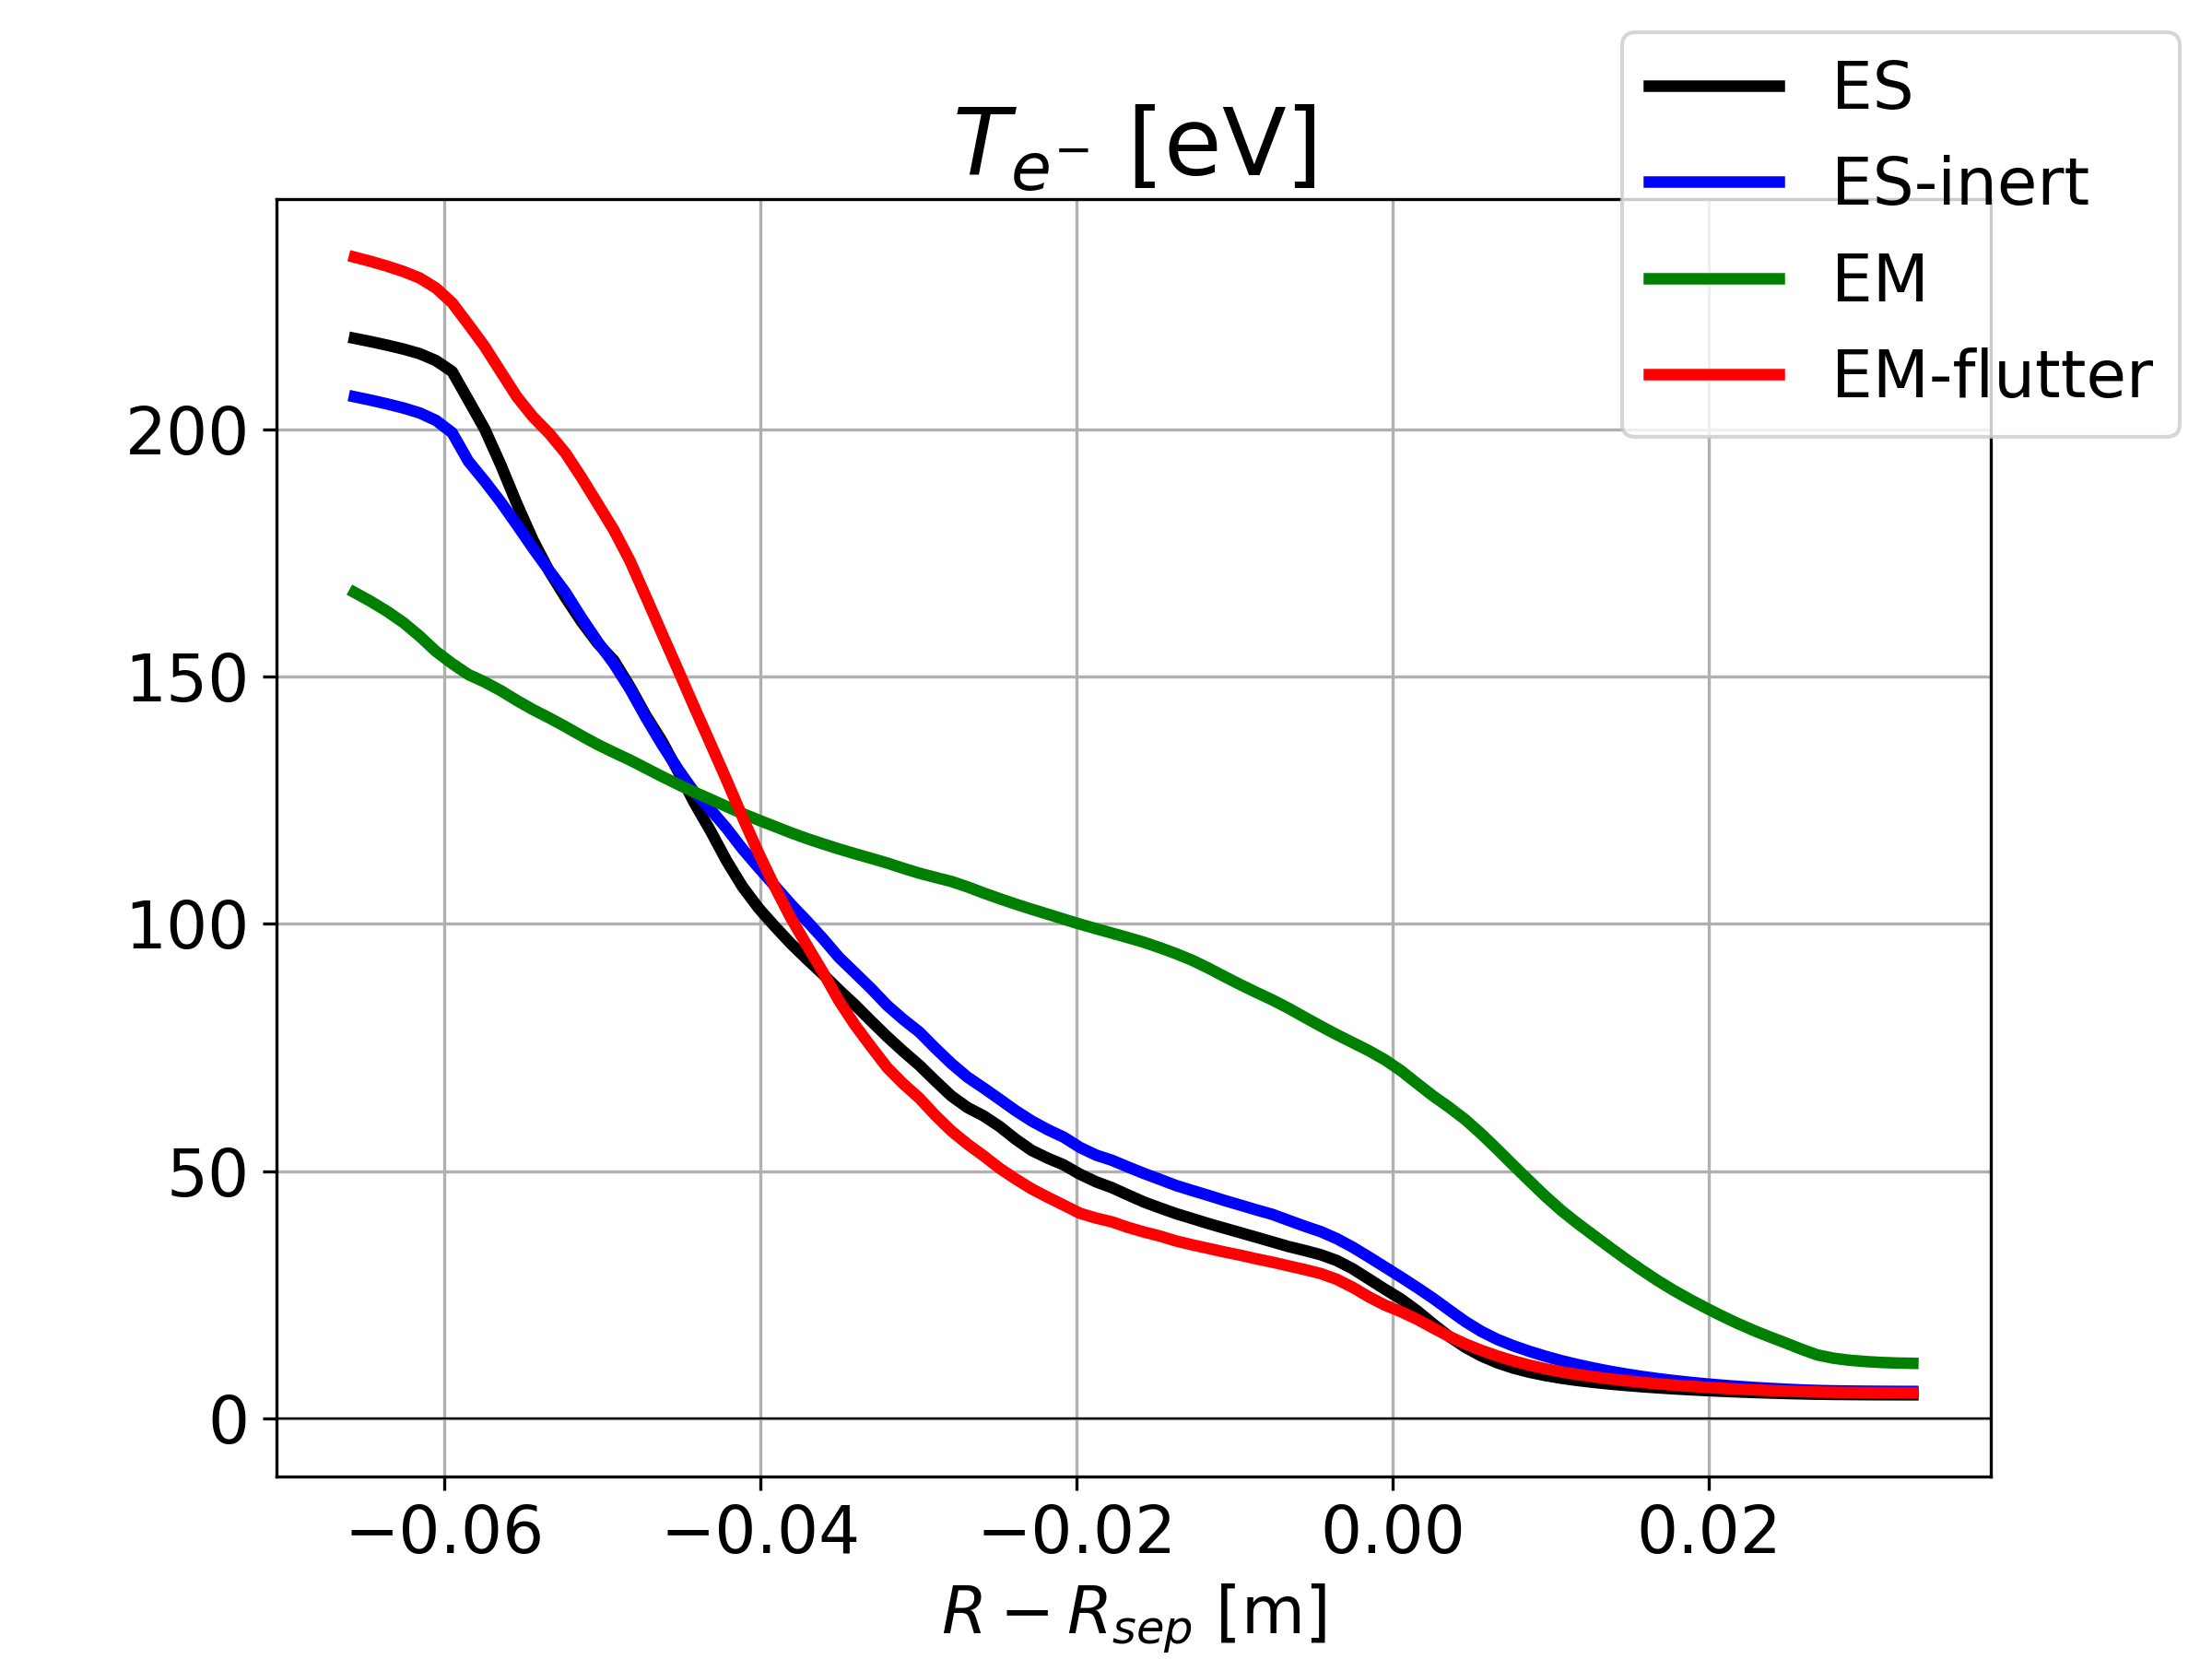
\includegraphics[width=1\textwidth]{schemes/OMP_profiles_e-_T.png}
		\subcaption{Electron temperature $T_e$}
	\end{subfigure}
	\begin{subfigure}[t]{0.30\textwidth}
		\centering
		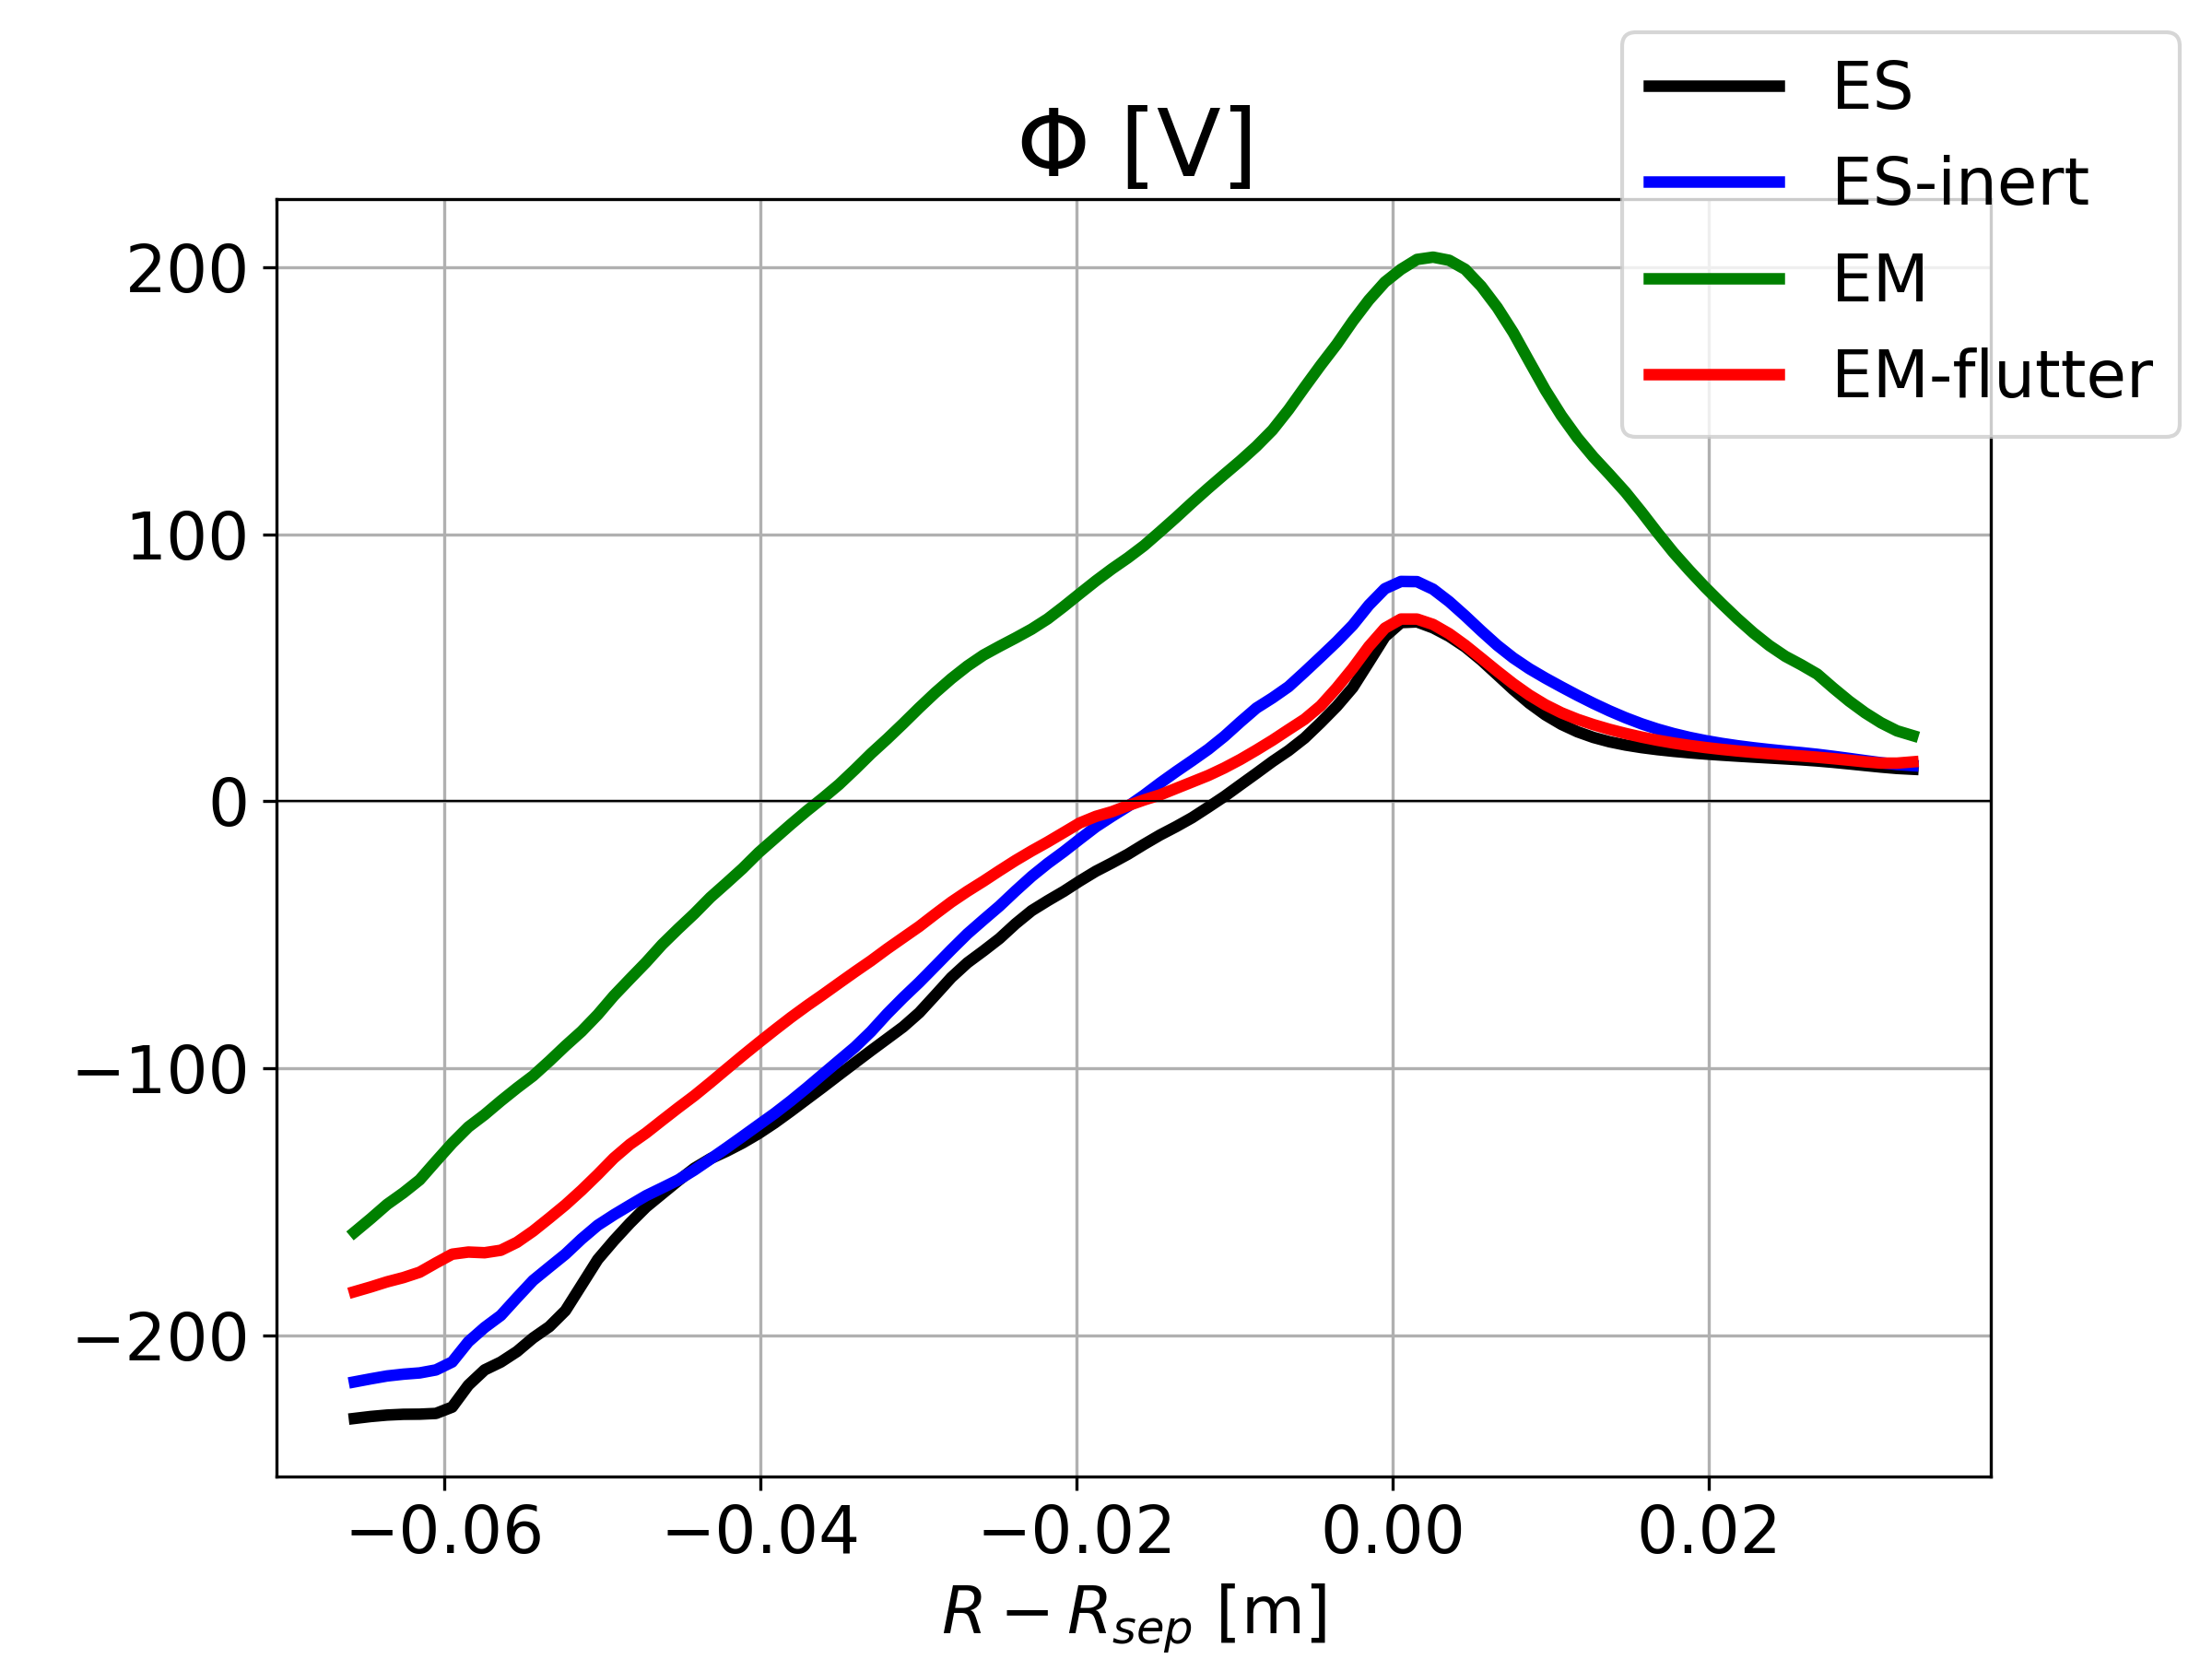
\includegraphics[width=1\textwidth]{schemes/OMP_profiles_global_fields_PHI.png}
		\subcaption{Electric potential $\Phi$}
	\end{subfigure}
	\caption[Radial profiles at the outer mid-plane after 6 ms simulated plasma time]{Radial profiles at the outer mid-plane after 6 ms simulated plasma time. These profiles were obtained by averaging simulation data across all 32 toroidal planes and over the last 20 available plasma saves.}
	\label{fig:OMP_profiles}
\end{figure}



\subsection{Numerical performances}
\label{performances}

In previous works about the electrostatic model\cite{tamain2016tokam3x, Bufferand2021}, it was pointed out that solving the implicit 3D vorticity operator is the most expensive and tricky operation in the algorithm. Adding new variables inevitably modifies the code's performance. With the rather coarse mesh used in the present work, simulations have been run on 16 nodes with 48 CPUs each on the MARCONI supercomputer operated by CINECA \cite{iannone2018marconi-fusion}. Implicit systems, such as the 3D vorticity operator, have been inverted using the stabilized biconjugate gradient method (BCGS) \cite{vandervorst1992bicgstab} with the generalized algebraic multigrid preconditioner (GAMG) by PETSc \cite{petsc-web-page}. \newline

The overall performance of the code largely depends on how quickly a certain plasma timespan can be calculated. Table \ref{tab:performanceMetric} presents the average simulation time for one timestep, broken down by the cost of each implicit solver. For the vorticity system, we also provide the number of iterations the BCGS needed to match the imposed tolerance ($10^{-8}$), as it relates to the condition number of the matrix. This system has always accounted for a considerable share of the total execution time and was heavily modified with the new electromagnetic model. Finally, the timestep size is provided, as a higher timestep size can compensate a costlier problem because the desired simulation time is reached in fewer iterations. As described earlier in Chap. \ref{chap:Implementation}, SOLEDGE3X uses a variable timestep scheme to maximize the CFL condition with the calculated fluxes. \newline

\begin{table}[h!]
	\centering
	\makebox[\textwidth][c]{
		\begin{tabularx}{1.13\textwidth}{|X|>{\centering\arraybackslash}p{0.12\textwidth}|>{\centering\arraybackslash}p{0.12\textwidth}|>{\centering\arraybackslash}p{0.12\textwidth}|>{\centering\arraybackslash}p{0.12\textwidth}|>{\centering\arraybackslash}p{0.12\textwidth}|>{\centering\arraybackslash}p{0.12\textwidth}|}
			\hline
			& Total execution time per timestep [ms] & Execution time for the viscosity [ms]  & Execution time for the heat diffusion [ms] & Execution time for the vorticity [ms] & N° of vorticity solver iterations & Timestep size [ns]  \\
			\hline
			\textbf{ES}         & 664  & 61  & 76  & 339  & 80  & 15.6 \\
			\hline    
			\textbf{ES-inert}   & 523  & 61  & 77  & 193  & 32  & 16.4 \\
			\hline    
			\textbf{EM}         & 895  & 63  & 82  & 552  & 60  & 15.9 \\
			\hline    
			\textbf{EM-flutter} & 2019 & 225 & 390 & 1147 & 55  & 16.6 \\
			\hline  
		\end{tabularx}
	}	
	\caption[Numerical metrics on the four TCV scenarios for one timestep]{Numerical metrics on the four TCV scenarios for one timestep. All quantities are averaged over the last 20000 timesteps of the simulation. The execution time refers to the wall-clock time and must be multiplied by the number of used processors (768) to get the actual used CPU time.}
	\label{tab:performanceMetric}
\end{table}

The introduction of a finite electron mass to the vorticity system significantly reduces the number of solver iterations and allows to reach a solution much faster. This improvement occurs because electron inertia effects dominate Ohm's law, thereby reducing the anisotropy between the perpendicular and parallel Laplacians on $\Phi$ in the electrostatic scenario. This reduction in anisotropy is due to the parallel diffusion coefficient being the conductivity $\sigma_\parallel$ in the electrostatic case, but a finite electron mass $m_e$ imposes an upper limit on it. Adding $A_\parallel$ doubles the size of the matrix and introduces a more complex structure, challenging the solvers and requiring more iterations. Despite the higher complexity, a finite electron mass allows the solver to converge in fewer iterations than in the reference electrostatic case. However, the effective solve time is still worse due to the doubling in system size. Finally, including flutter slightly improves the matrix condition compared to the scenario with only magnetic induction, but the execution time is significantly increased. At first glance, one would expect the solve time to correlate with the number of BCGS iterations as both electromagnetic scenarios solve a coupled 3D system on $\Phi$ and $A_\parallel$. Since flutter introduces the radial direction to parallel gradients, and the coupling terms between the two unknowns are exactly a parallel gradient and a divergence (see Eq. \ref{eq:impl_implicitVorticitySystem}), the matrix exhibits a decreased sparsity ratio. This circumstance is further aggravated by the fact that $A_\parallel$ is not staggered in the radial direction, so the radial discrete gradient/divergence operator has a larger stencil width than its poloidal and toroidal counterparts. \newline

The viscosity and heat diffusion solvers are not directly affected by the electromagnetic model, and their solve times are similar for the first three scenarios. Electromagnetic flutter, however, with its radial gradient (again), heavily modifies the parallel diffusion operators and requires solving one global 3D system instead of separate 2D systems on each flux surface (see Sec. \ref{ssec:impl_3DGunter}). This is immediately reflected in the code performance, as both solvers take up to 5 times longer to solve. \newline

In total, electron inertia decreases the computing time with an excellent improvement of the vorticity matrix condition. The magnetic inductive model means slightly higher computational costs, because the implicit vorticity problem doubles in size. Including electromagnetic flutter in the system almost quadruples the execution time compared to the original implementation because the radial parallel gradient complicates both the implicit vorticity and the parallel diffusion problem. The timestep size does not vary considerably between the scenarios and hence has only a limited impact on the overall performance.


\section{Flutter in higher power}

In the previous section, we compared the new electromagnetic model in an L-mode scenario inspired by the TCV-X21 benchmark. Electromagnetic effects scale with the pressure ratio $\beta$, so it would be more than interesting to study electromagnetic plasma behavior. The main difference to the previous set-up is a constant heat source of 1.2MW equally distributed among ions and electrons at the core boundary. For higher fidelity, we also replace the fixed particle source by interaction with fluid neutrals using the most recent implemented model\cite{quadri2024}. However, this simulation setup is not entirely realistic, as at such high power, substantial external heating is applied to the edge plasma, and we cannot assume that all of it originates from the unsimulated core. Moreover, thresholding issues with the neutral model lead to an excessive particle source in the core, distorting density profiles. For this study we only consider the full model with magnetic induction, electron inertia and flutter.  \\



\subsection{Parallel heat conduction}

Akin the simple magnetic inductive scenario the low-power scenario, the system reaches rapidly a quasi-steady state after 3ms. However, there is no uncontrolled collapse of the density and temperature in the core, at the contrary, steep gradients build up in the edge and just behind the separatrix. In the SOL, gradients are very small up to the first wall, leaving convenient low values throughout the region. This can be observed in the outer-mid plane profiles for ion density and temperature, taken at increasing simulation times in Fig. \ref{fig:TCV_highPower_OMP}. \\

The temperature profile could indicate the formation of a pedestal, characteristic of the transport barrier in H-mode plasmas with an improved confinement quality. To properly assess such a condition, the simulation must however reach a full steady state, especially on the density, whose confinement time is much higher and far beyond the end of this simulation. \\

\begin{figure}[H]\centering
	\begin{subfigure}[t]{0.45\textwidth}
		\centering
		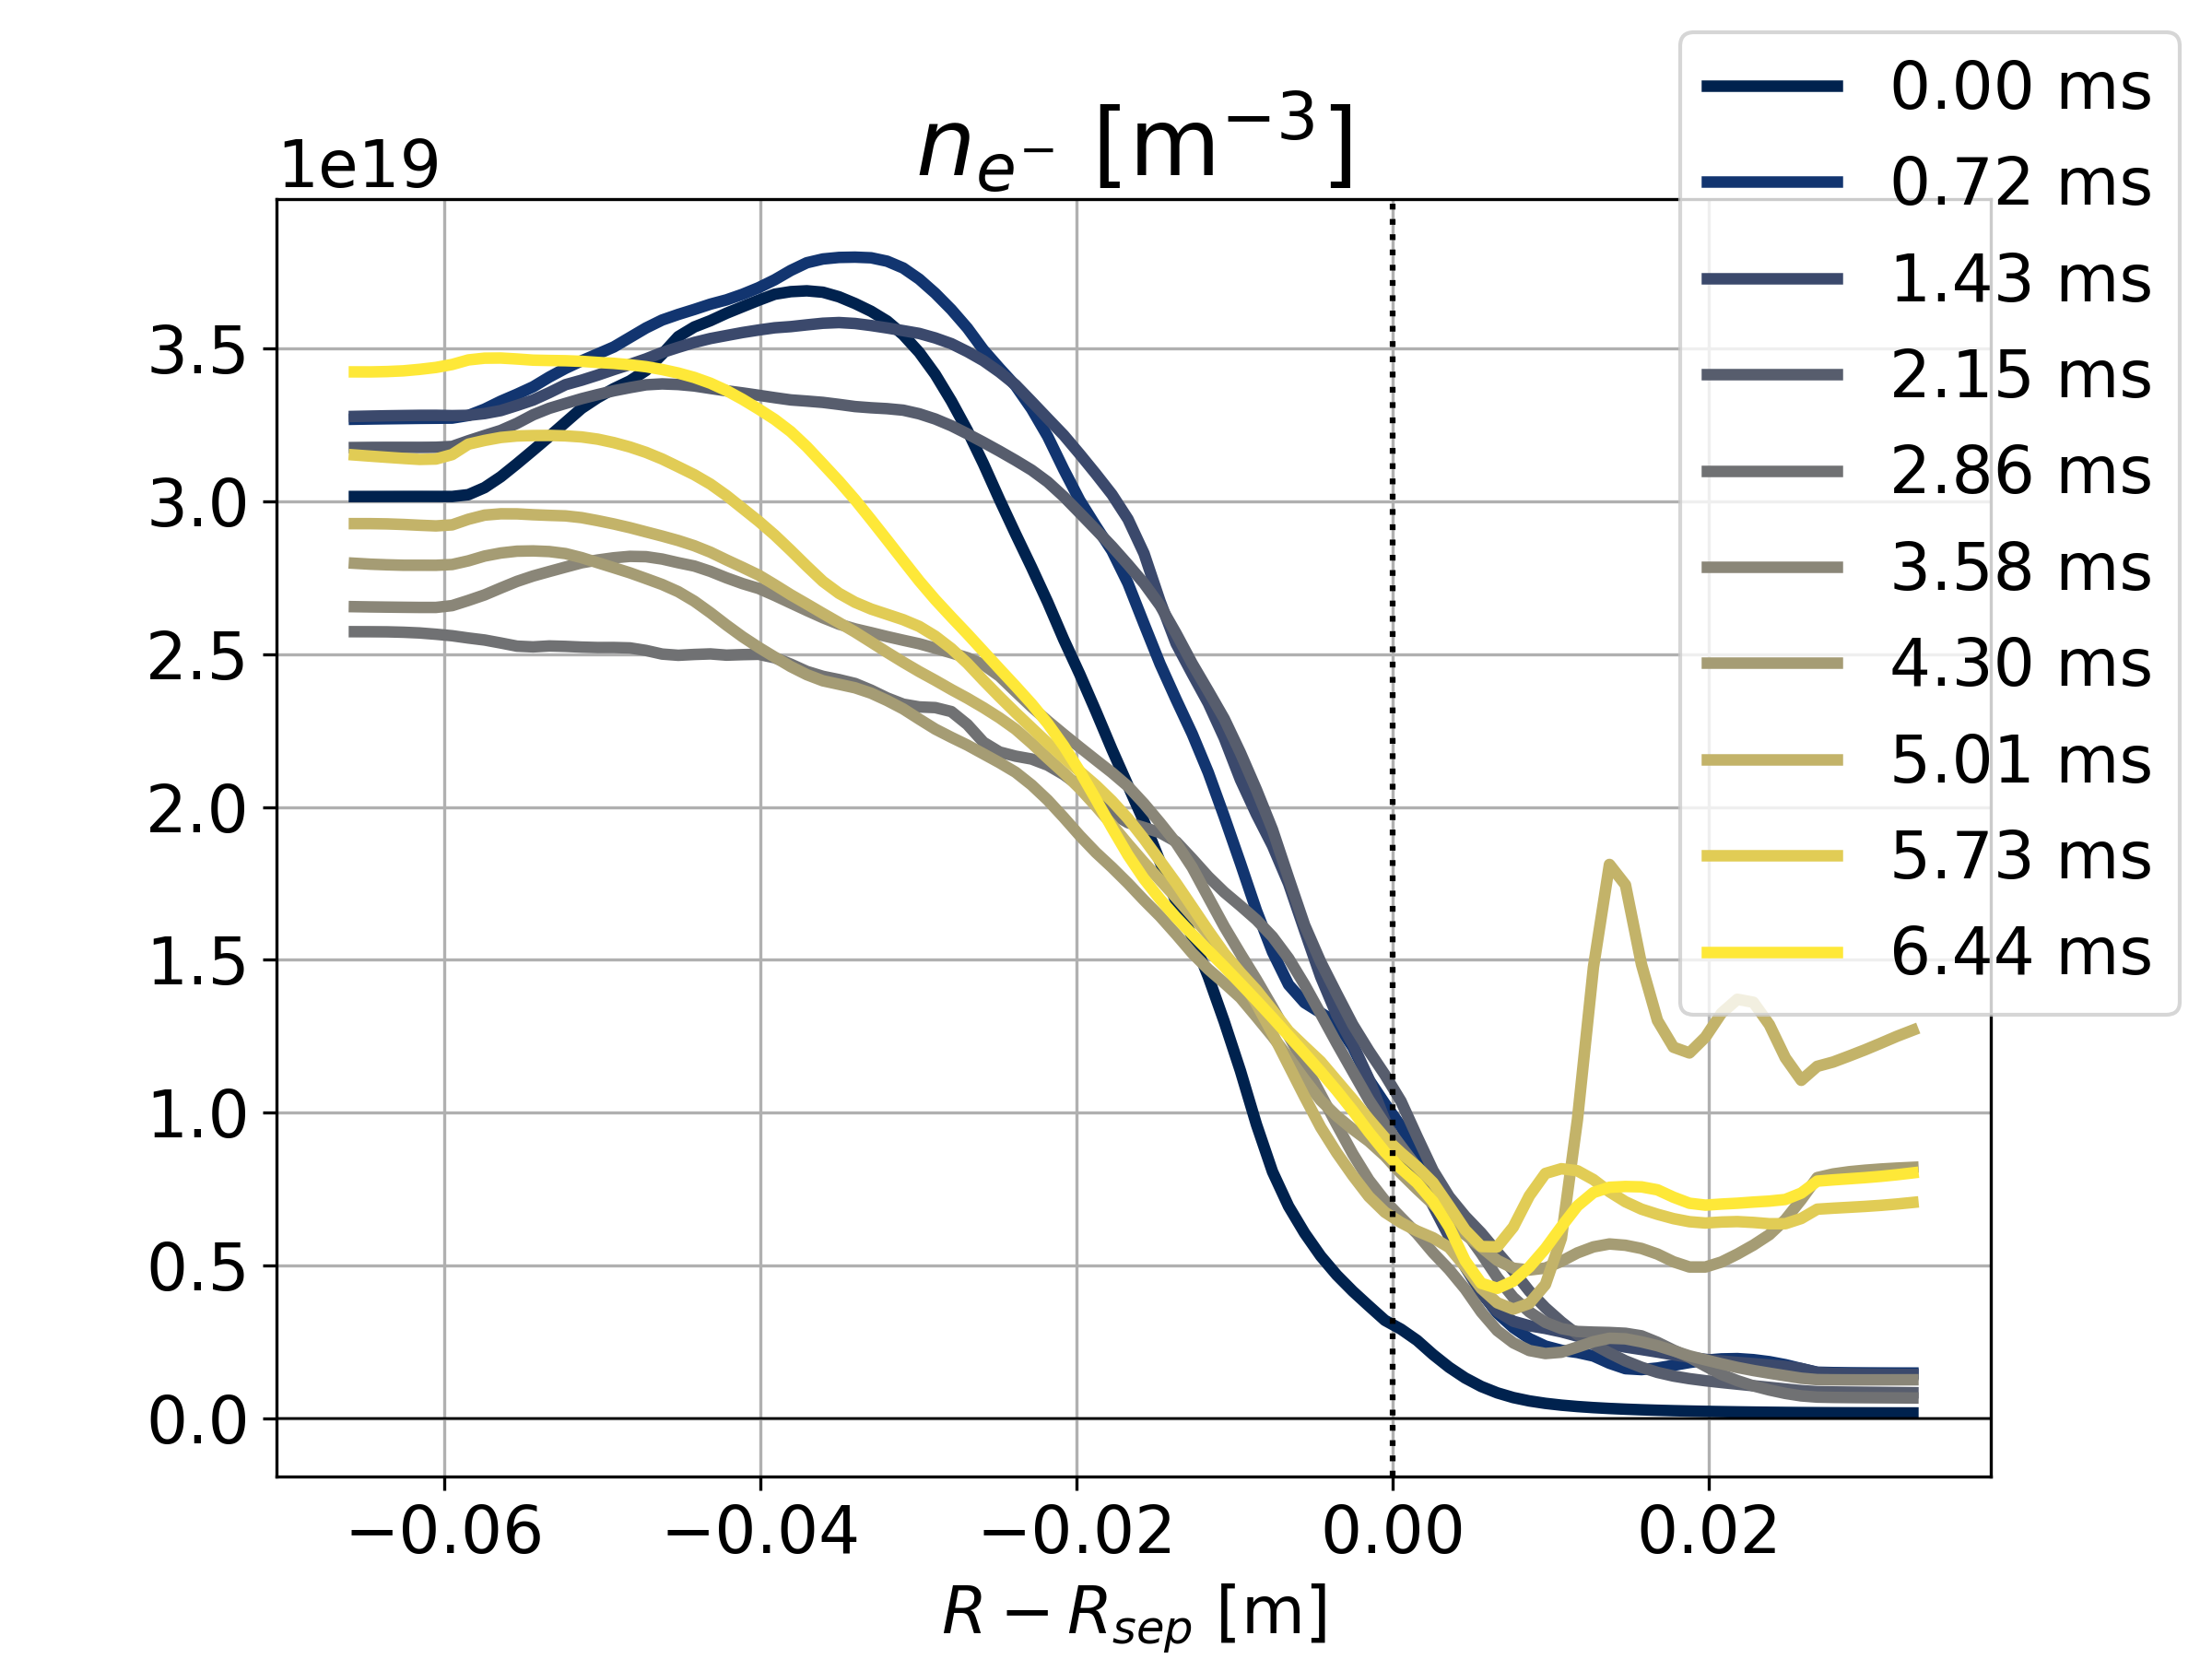
\includegraphics[width=1\textwidth]{schemes/OMP_profiles_e-_n_Hmode.png}
		\subcaption{Ion density}
		\label{fig:TCV_highPower_OMPn}
	\end{subfigure}
	\begin{subfigure}[t]{0.45\textwidth}
		\centering
		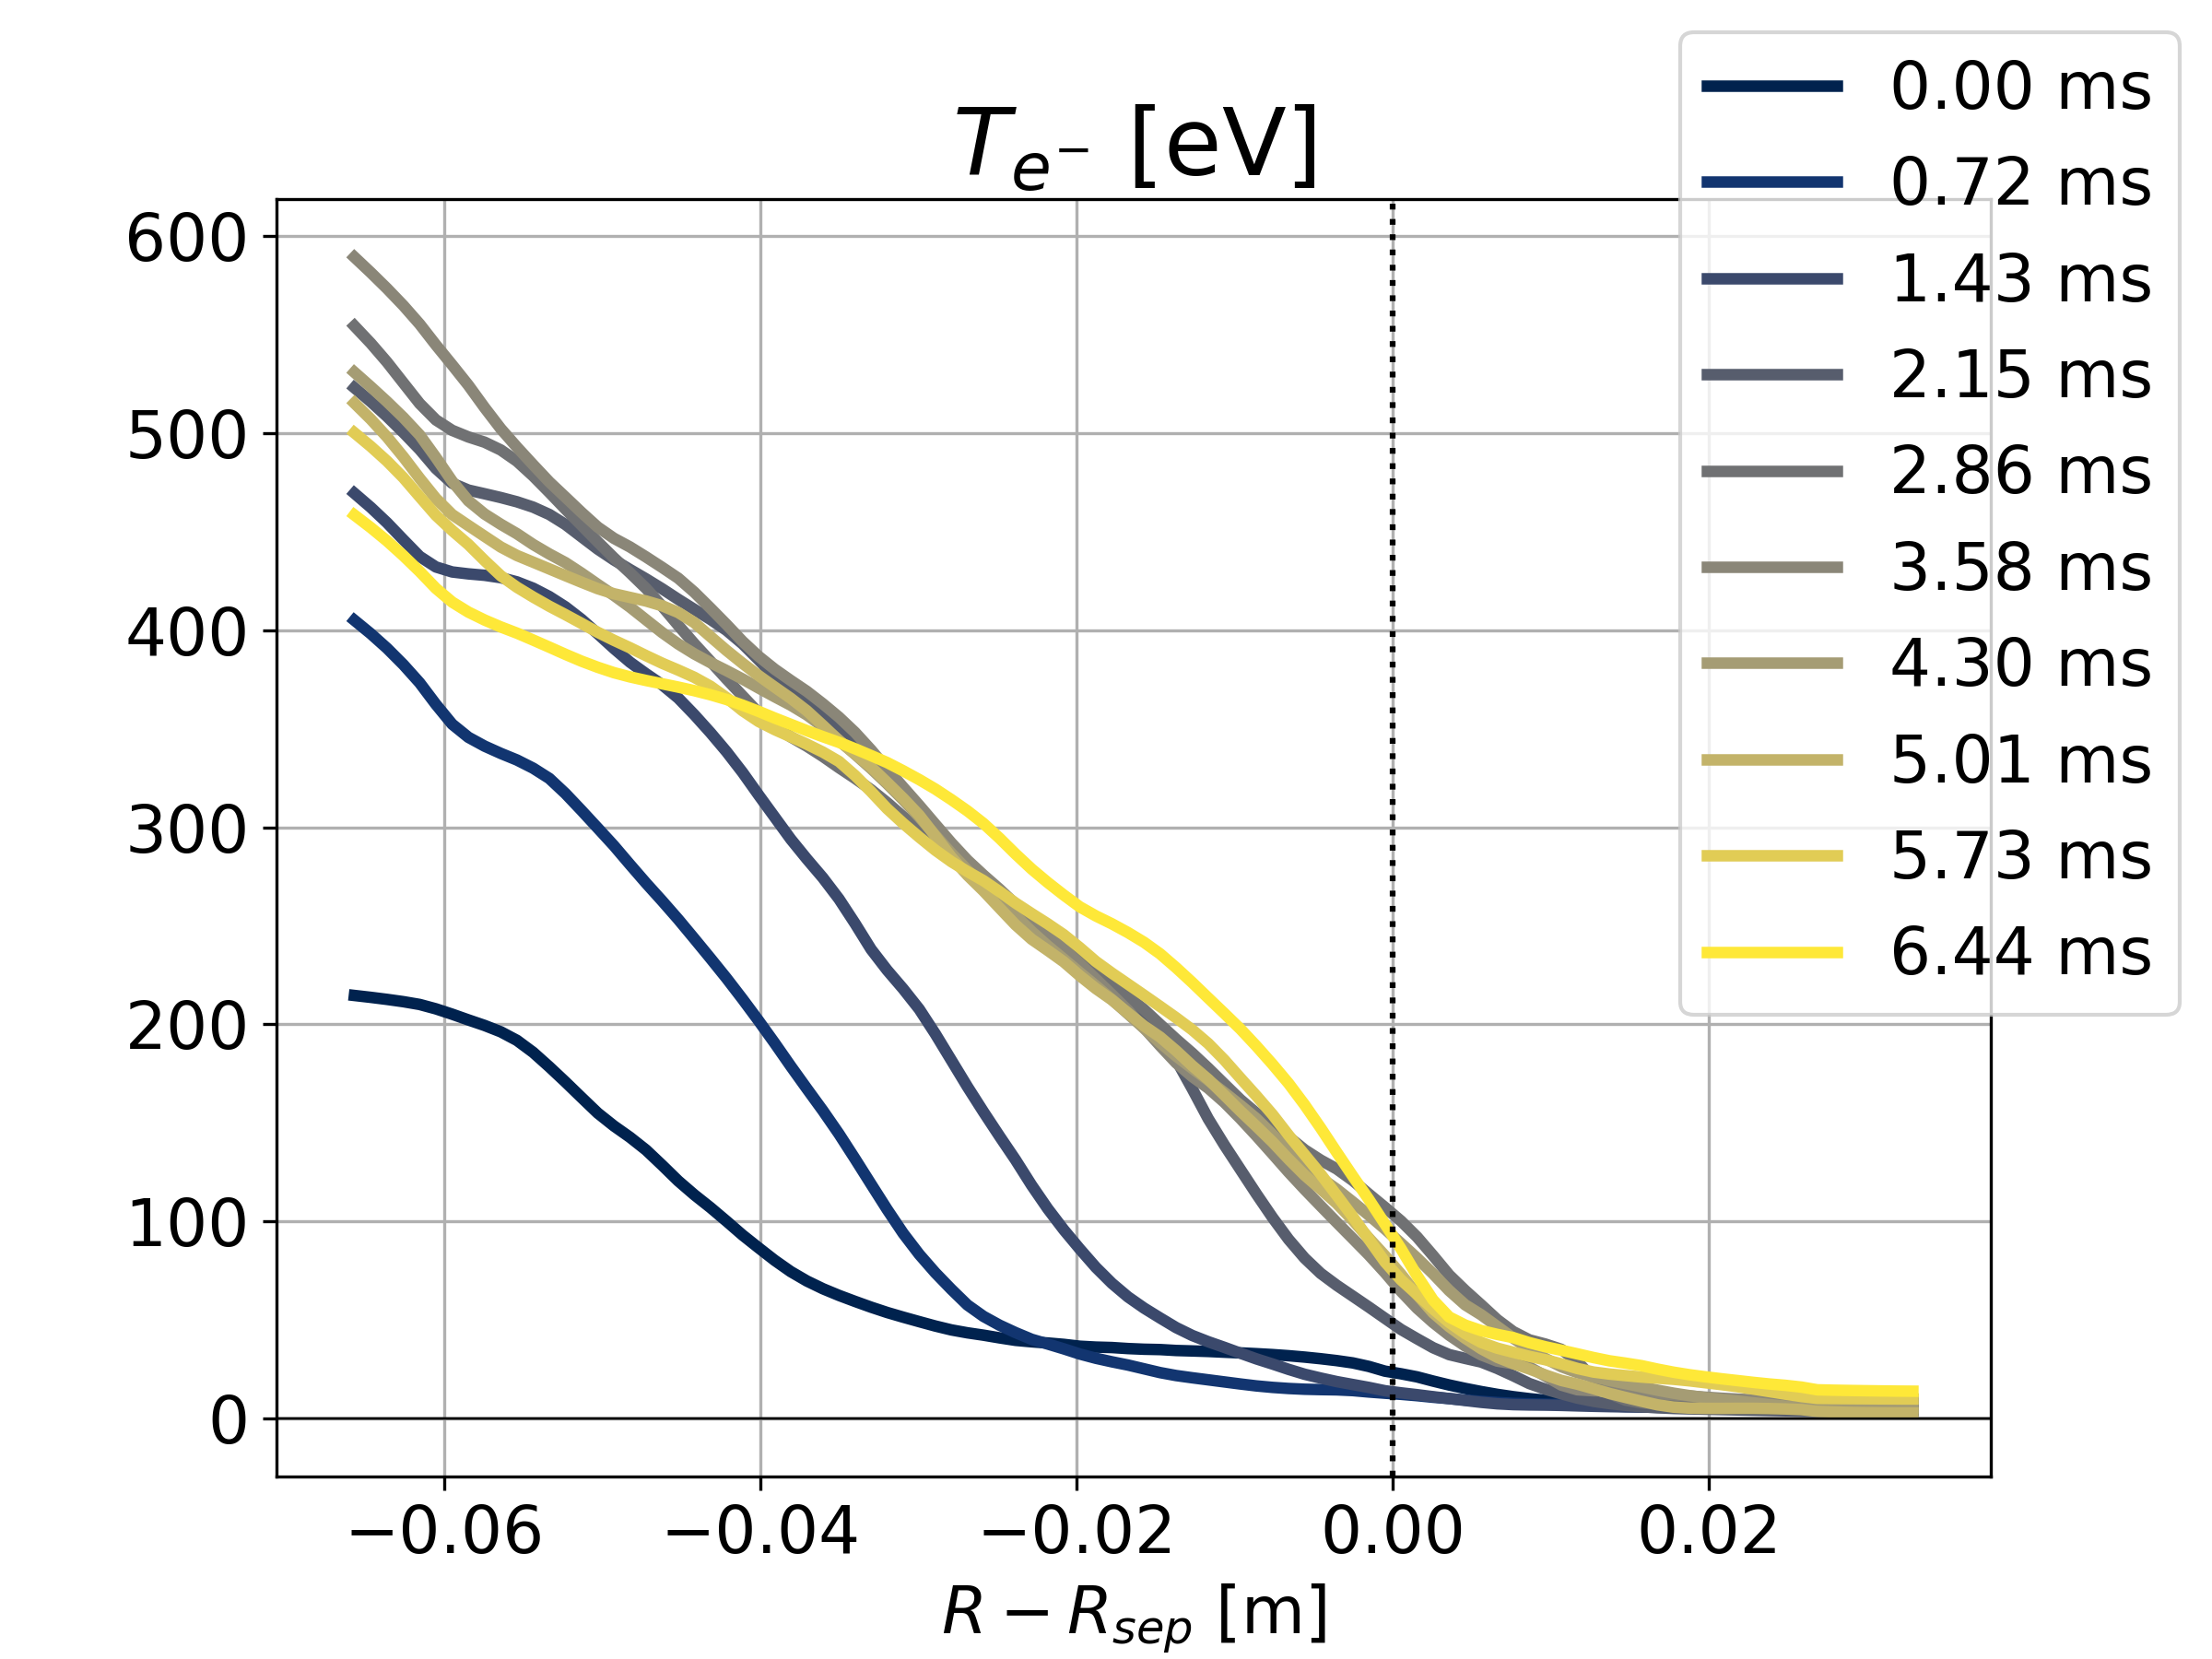
\includegraphics[width=1\textwidth]{schemes/OMP_profiles_e-_T_Hmode.png}
		\subcaption{Ion temperature}
		\label{fig:TCV_highPower_OMPT}
	\end{subfigure}
	\caption[Averaged profiles at the outer mid plane taken at different simulation times for the TCV scenarion with a 1.2MW heat source]{Averaged profiles at the outer mid plane taken at different simulation times for the TCV scenarion with a 1.2MW heat source.}
	\label{fig:TCV_highPower_OMP}
\end{figure}

We can still investigate heat fluxes to understand the behavior of the temperature. Let us examine the components to the total heat flux at the separatrix, as they will ultimately define the confinement of the core plasma. For that, we have a closer look to the different contributions to the radial heat flux in the energy conservation equation. The main terms are advection of thermal and kinetic plasma energy by electric and curvature drifts as well as the radial redirection of parallel fluxes due to flutter. The parallel heat conduction $q_\parallel$ now also contains a radial component. The contribution of the viscous fluxes vanishes for electrons and is negligible for the ion heat flux, so we do not consider it in our analysis. We can express the total radial power transfer from core to SOL as: 

\begin{equation}
	P_\psi^{sep} = \underbrace{\int_{sep} \mathbf{e}_\psi \cdot \varepsilon n \mathbf{u}^{ExB}_\psi dA_{sep}}_{\text{ExB}} + \underbrace{\int_{sep} \mathbf{e}_\psi \cdot \varepsilon n \mathbf{u}^{\grad B}_\psi dA_{sep}}_{\text{gradB}} + \underbrace{\int_{sep} \mathbf{e}_\psi \cdot \varepsilon n v_\parallel \mathbf{b}_\psi dA_{sep}}_{\text{EM}} + \underbrace{\int_{sep} \mathbf{e}_\psi\cdot\left[-\kappa_{SH} \grad_\parallel T\mathbf{b}_\psi\right] dA_{sep}}_{\text{qpara}}
\end{equation}

In Fig. \ref{fig:TCV_decompHeatFluxFlutter}, we compare the evolution of each individual term to the total power the over the simulation time, integrated over the entire separatrix flux surface. The simulation outputs were also scaled by a factor four to express the power on the full torus (and not only the simulated quarter).

\begin{figure}[H]\centering
	\begin{subfigure}[t]{0.45\textwidth}
		\centering
		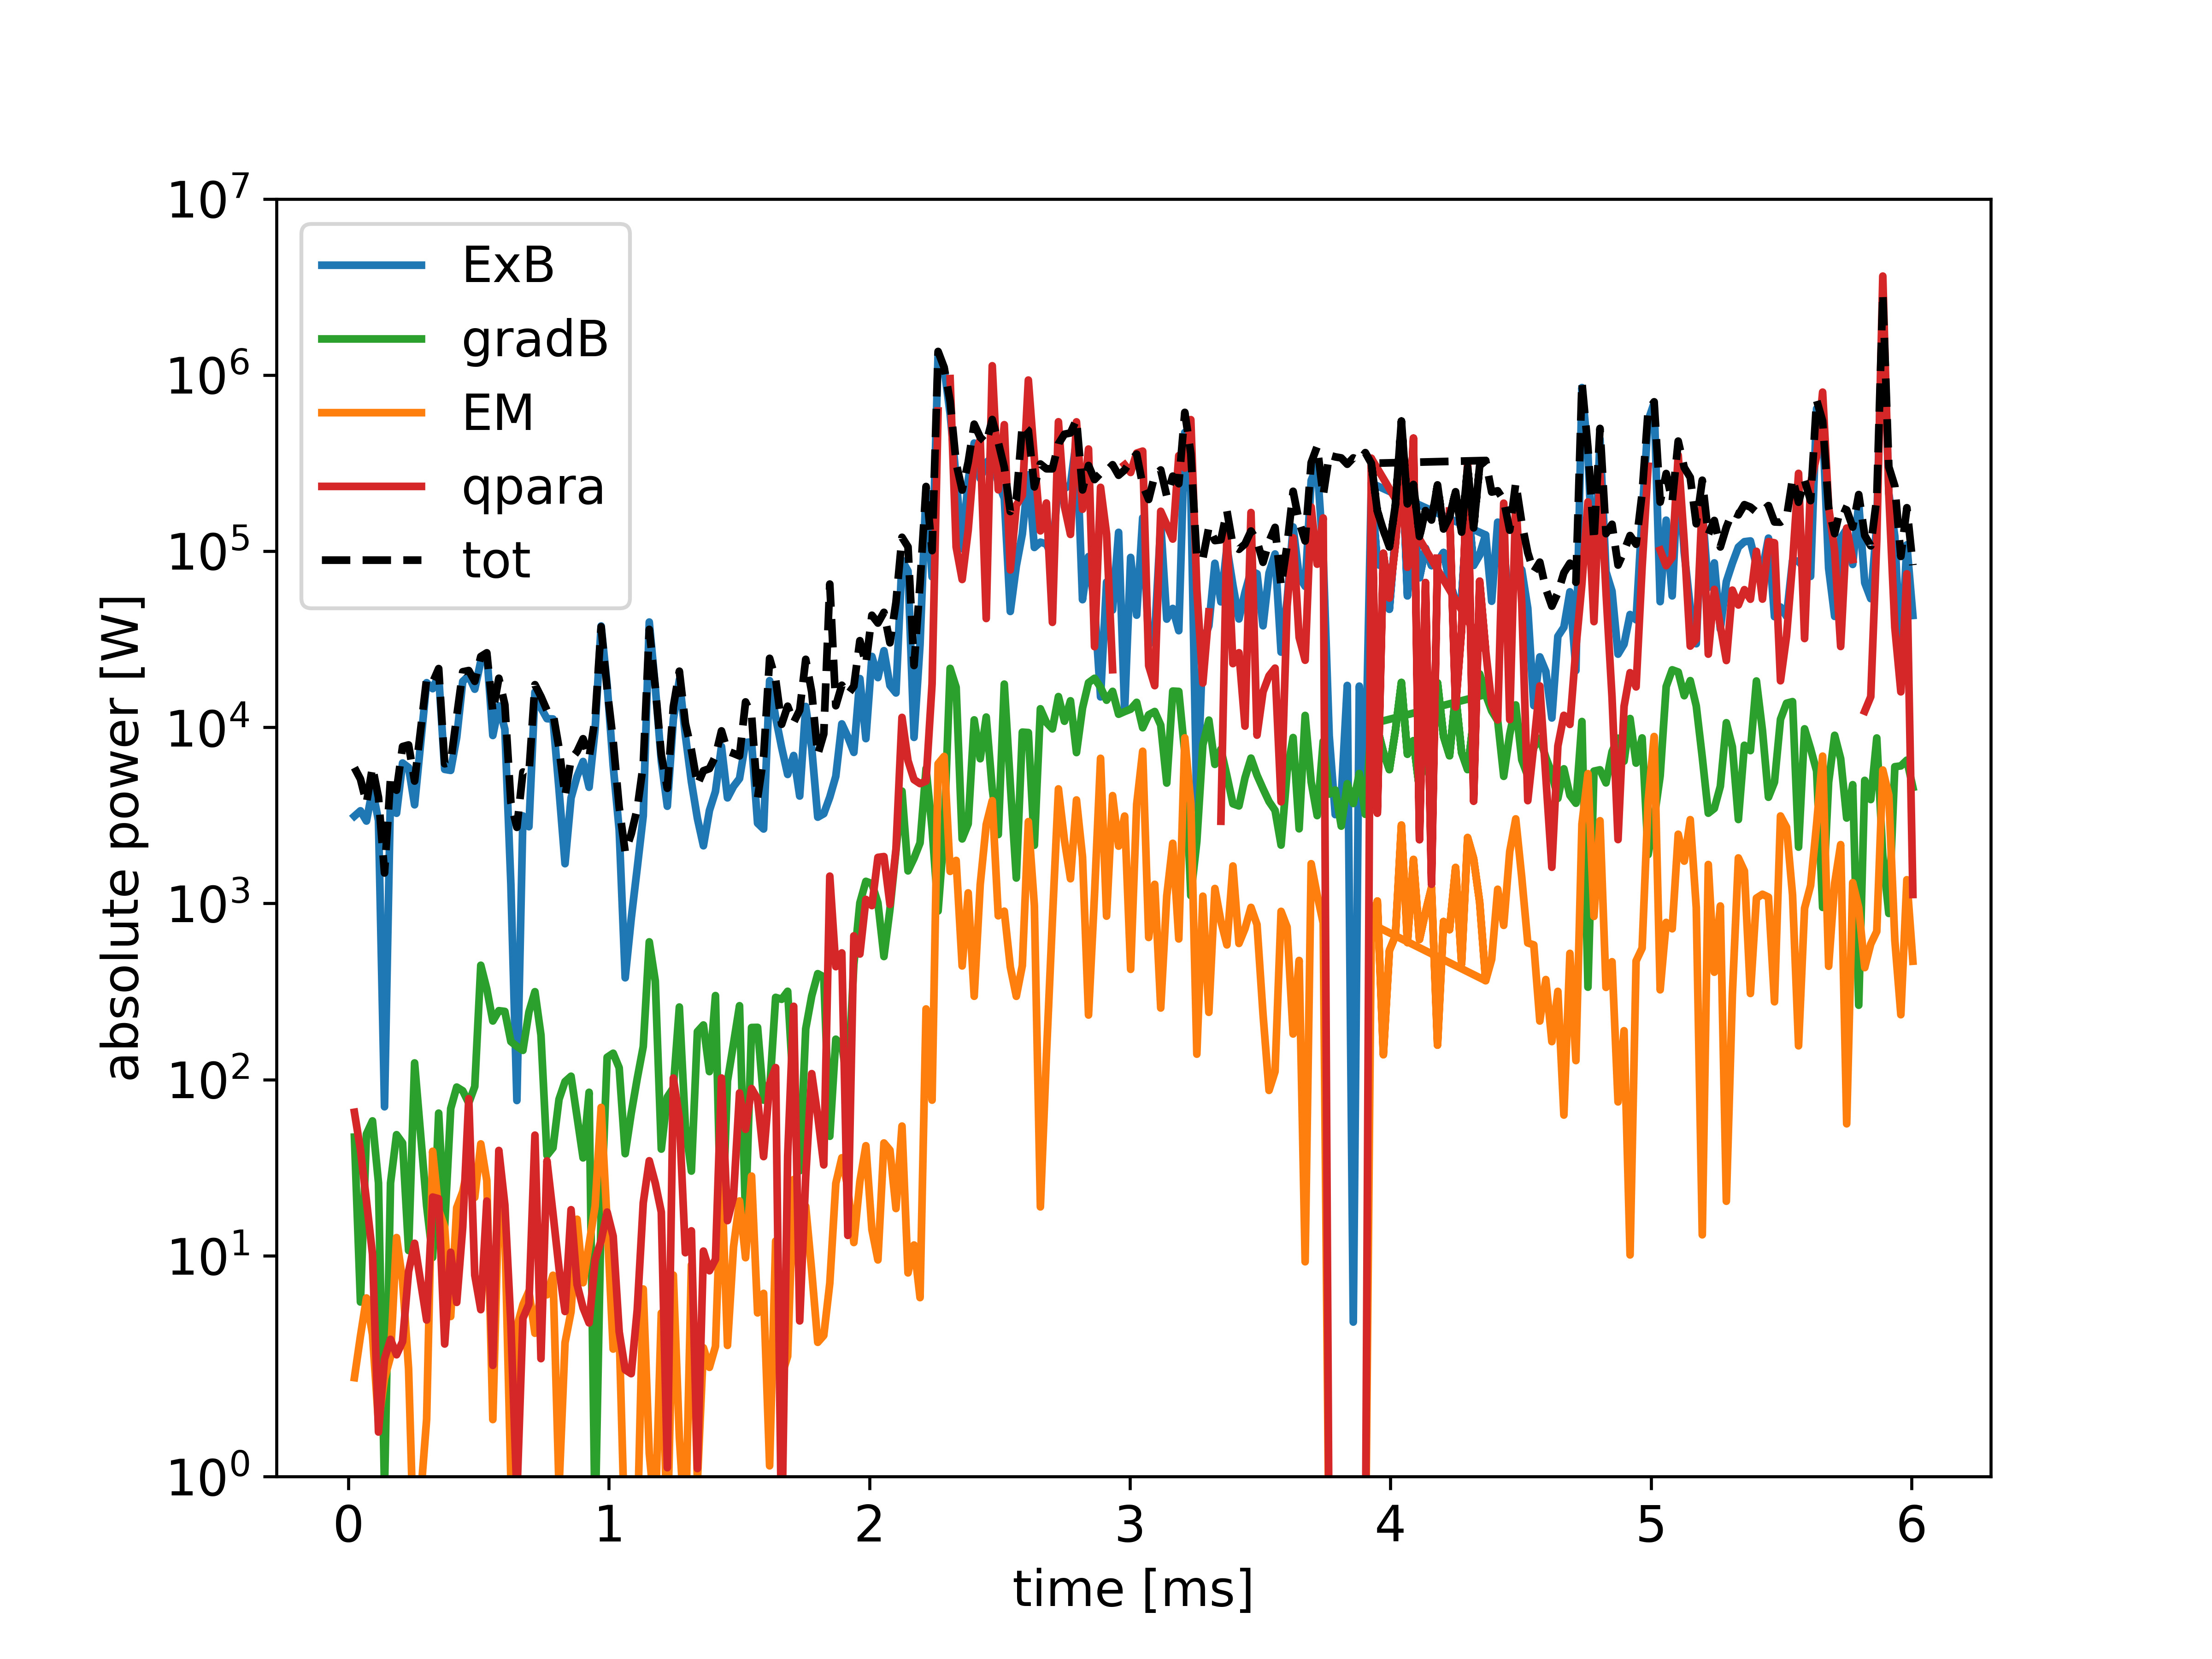
\includegraphics[width=1\textwidth]{schemes/heatflux_comp_sepc_spec0.jpg}
		\subcaption{Electron power flux}
		\label{fig:TCV_decompHeatFluxFlutter_electron}
	\end{subfigure}
	\begin{subfigure}[t]{0.45\textwidth}
		\centering
		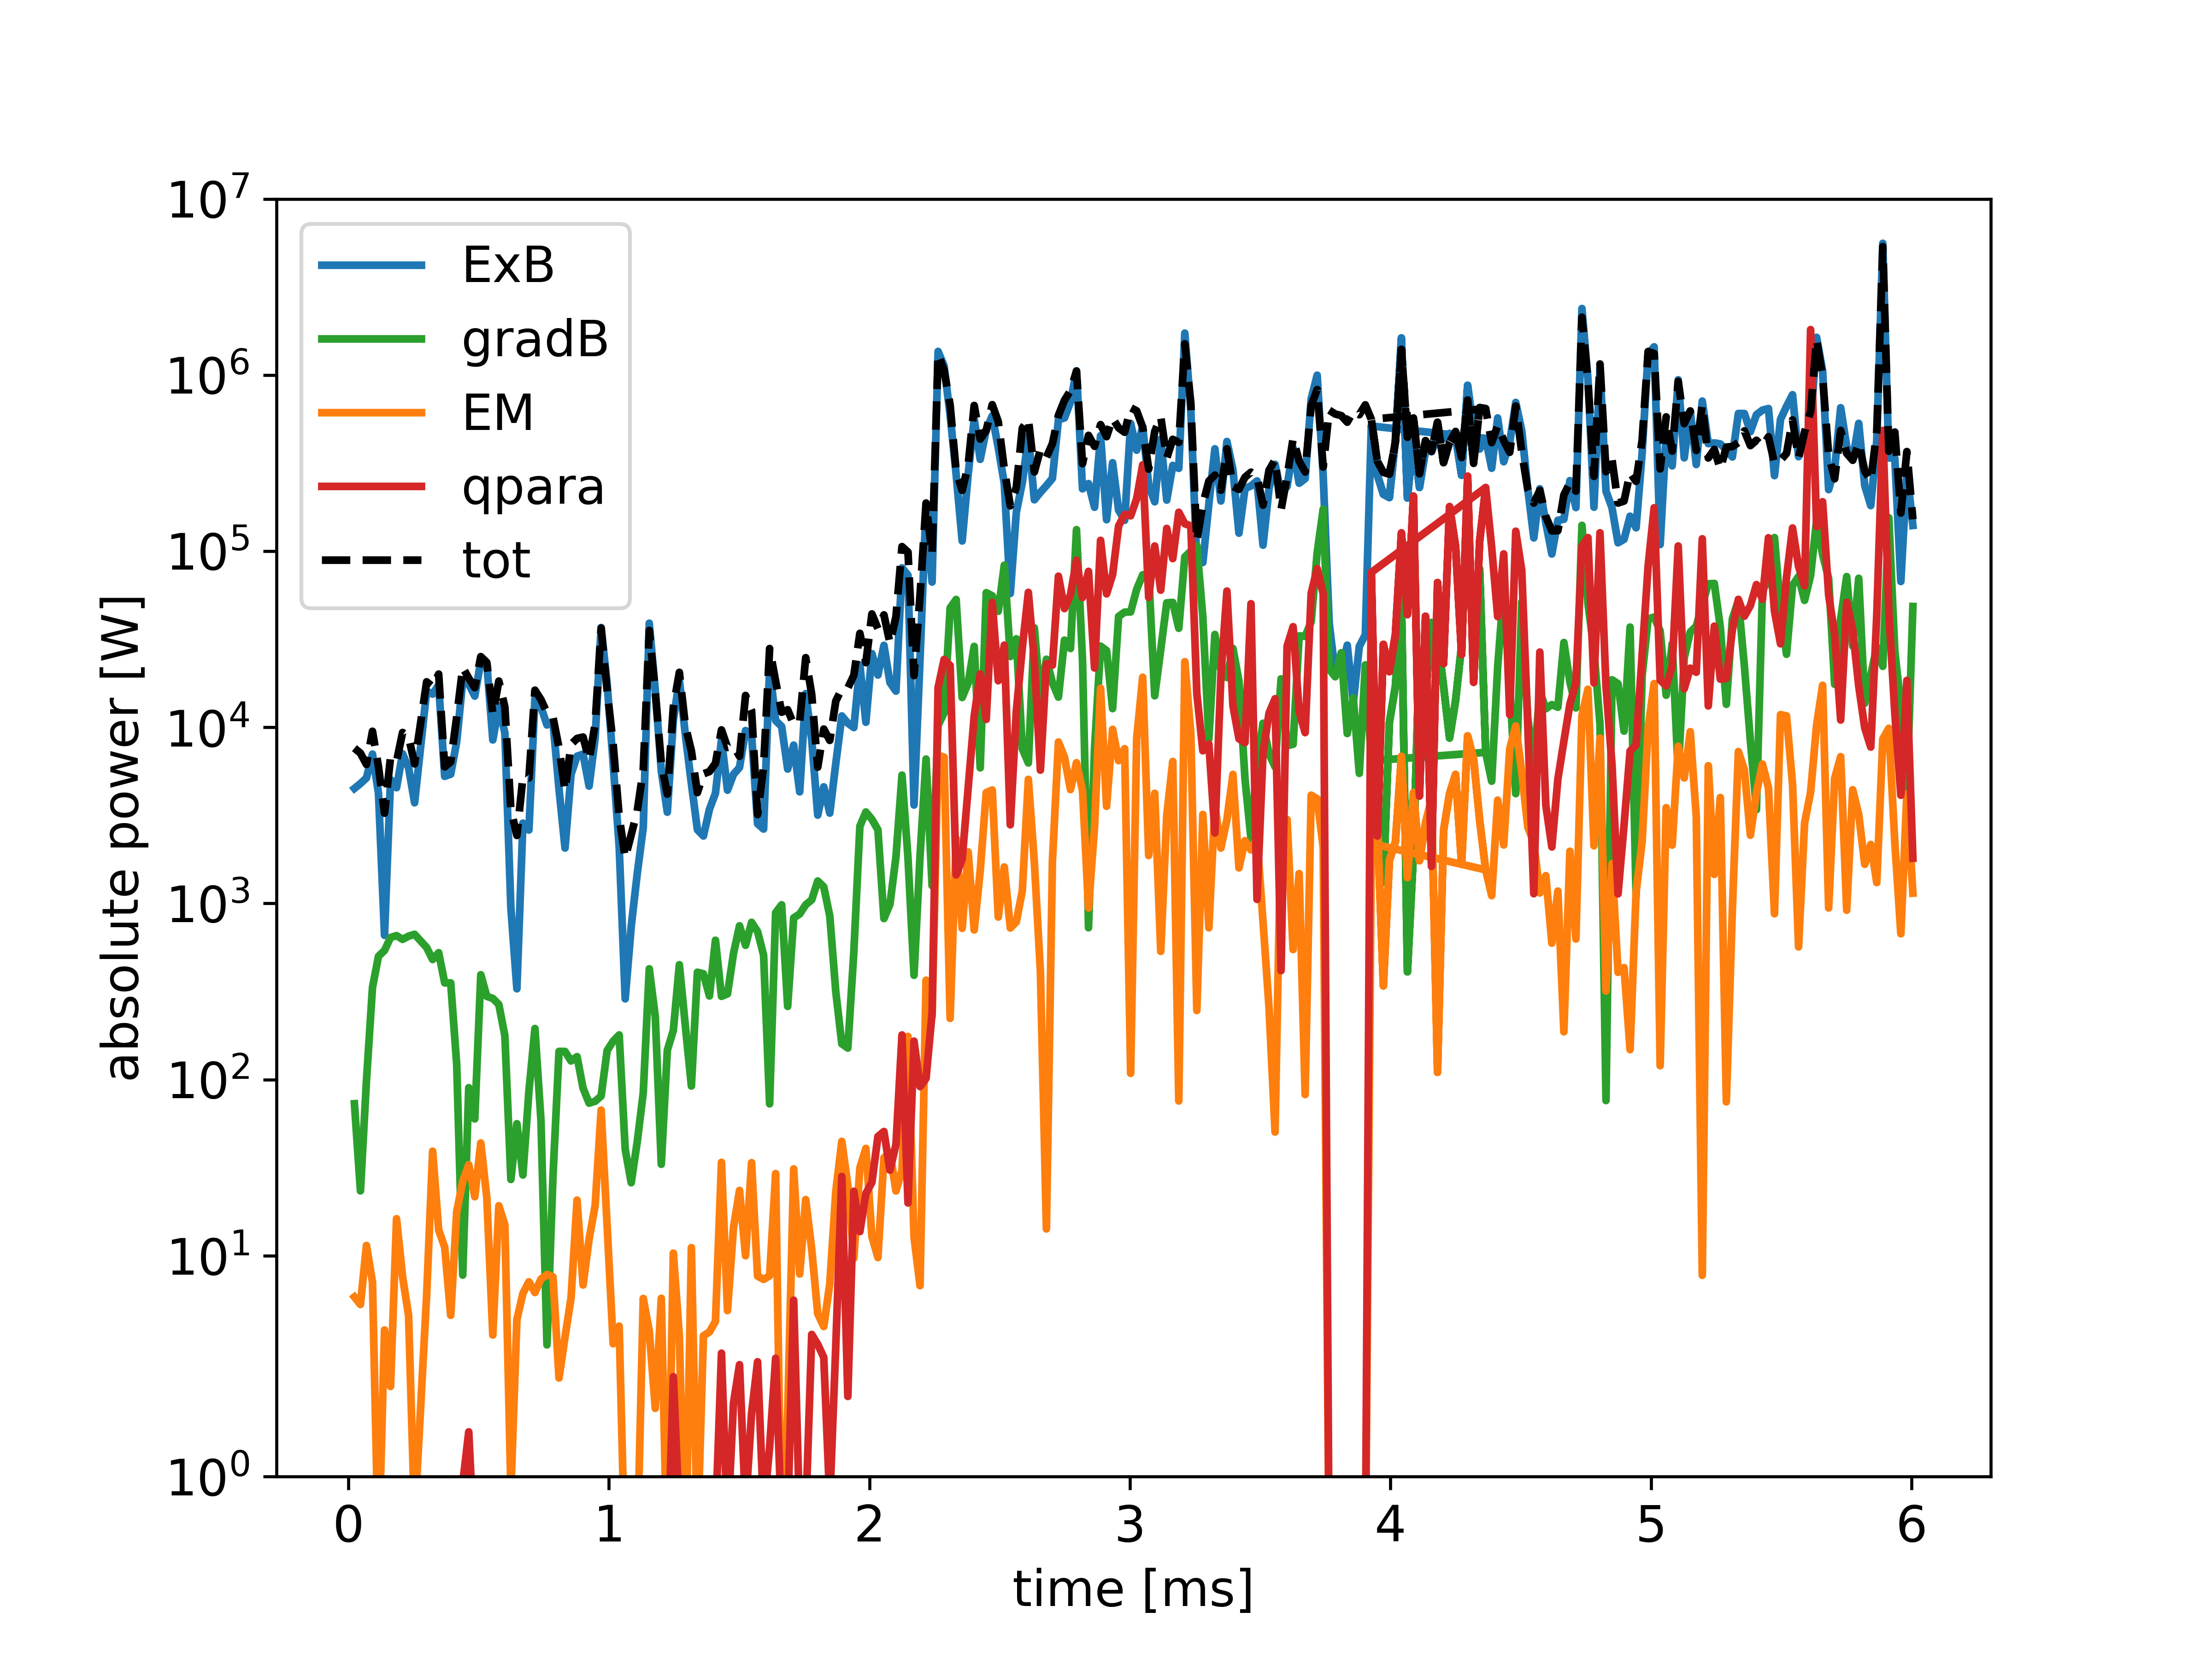
\includegraphics[width=1\textwidth]{schemes/heatflux_comp_sepc_spec1.jpg}
		\subcaption{Ion power flux}
		\label{fig:TCV_decompHeatFluxFlutter_ion}
	\end{subfigure}
	\caption[Contribution of the different terms in the energy conservation equation to the power transfer from the core to the SOL]{Contribution of the different terms in the energy conservation equation to the power transfer from the core to the SOL.}
	\label{fig:TCV_decompHeatFluxFlutter}
\end{figure}





\subsection{Characteristics of the fluctuating field}

As electromagnetic transport in the tokamak edge starts to play a role, the time has come to investigate electromagnetic flutter a bit more in detail. 

\subsubsection{View of the flutter field}


Let us trace the perturbed field lines driven by flutter on the first poloidal plane at the end of the simulation. Fig. \ref{fig:TCV_poincareFlutter} shows the field lines starting at 2500 points seeded randomly across the entire domain. As the integration length for each line has been fixed beforehand, longer lines correlate with higher magnitudes of $\mathbf{\tilde{B}}$. This is not a true Poincaré plot however, as flutter also contains a toroidal component, that is much smaller than the other two components, but was neglected for this analysis. If it was included, field lines would immediately leave the plane of interest and only return sporadically, leaving not much more than the seed points on the Poincaré plot. It could also have been possible to create this plot for the full magnetic field, including the equilbrium component, but then it would have been utterly hard to distinguish unique features of flutter. \newline 

\begin{figure}[H]\centering
	\centering
	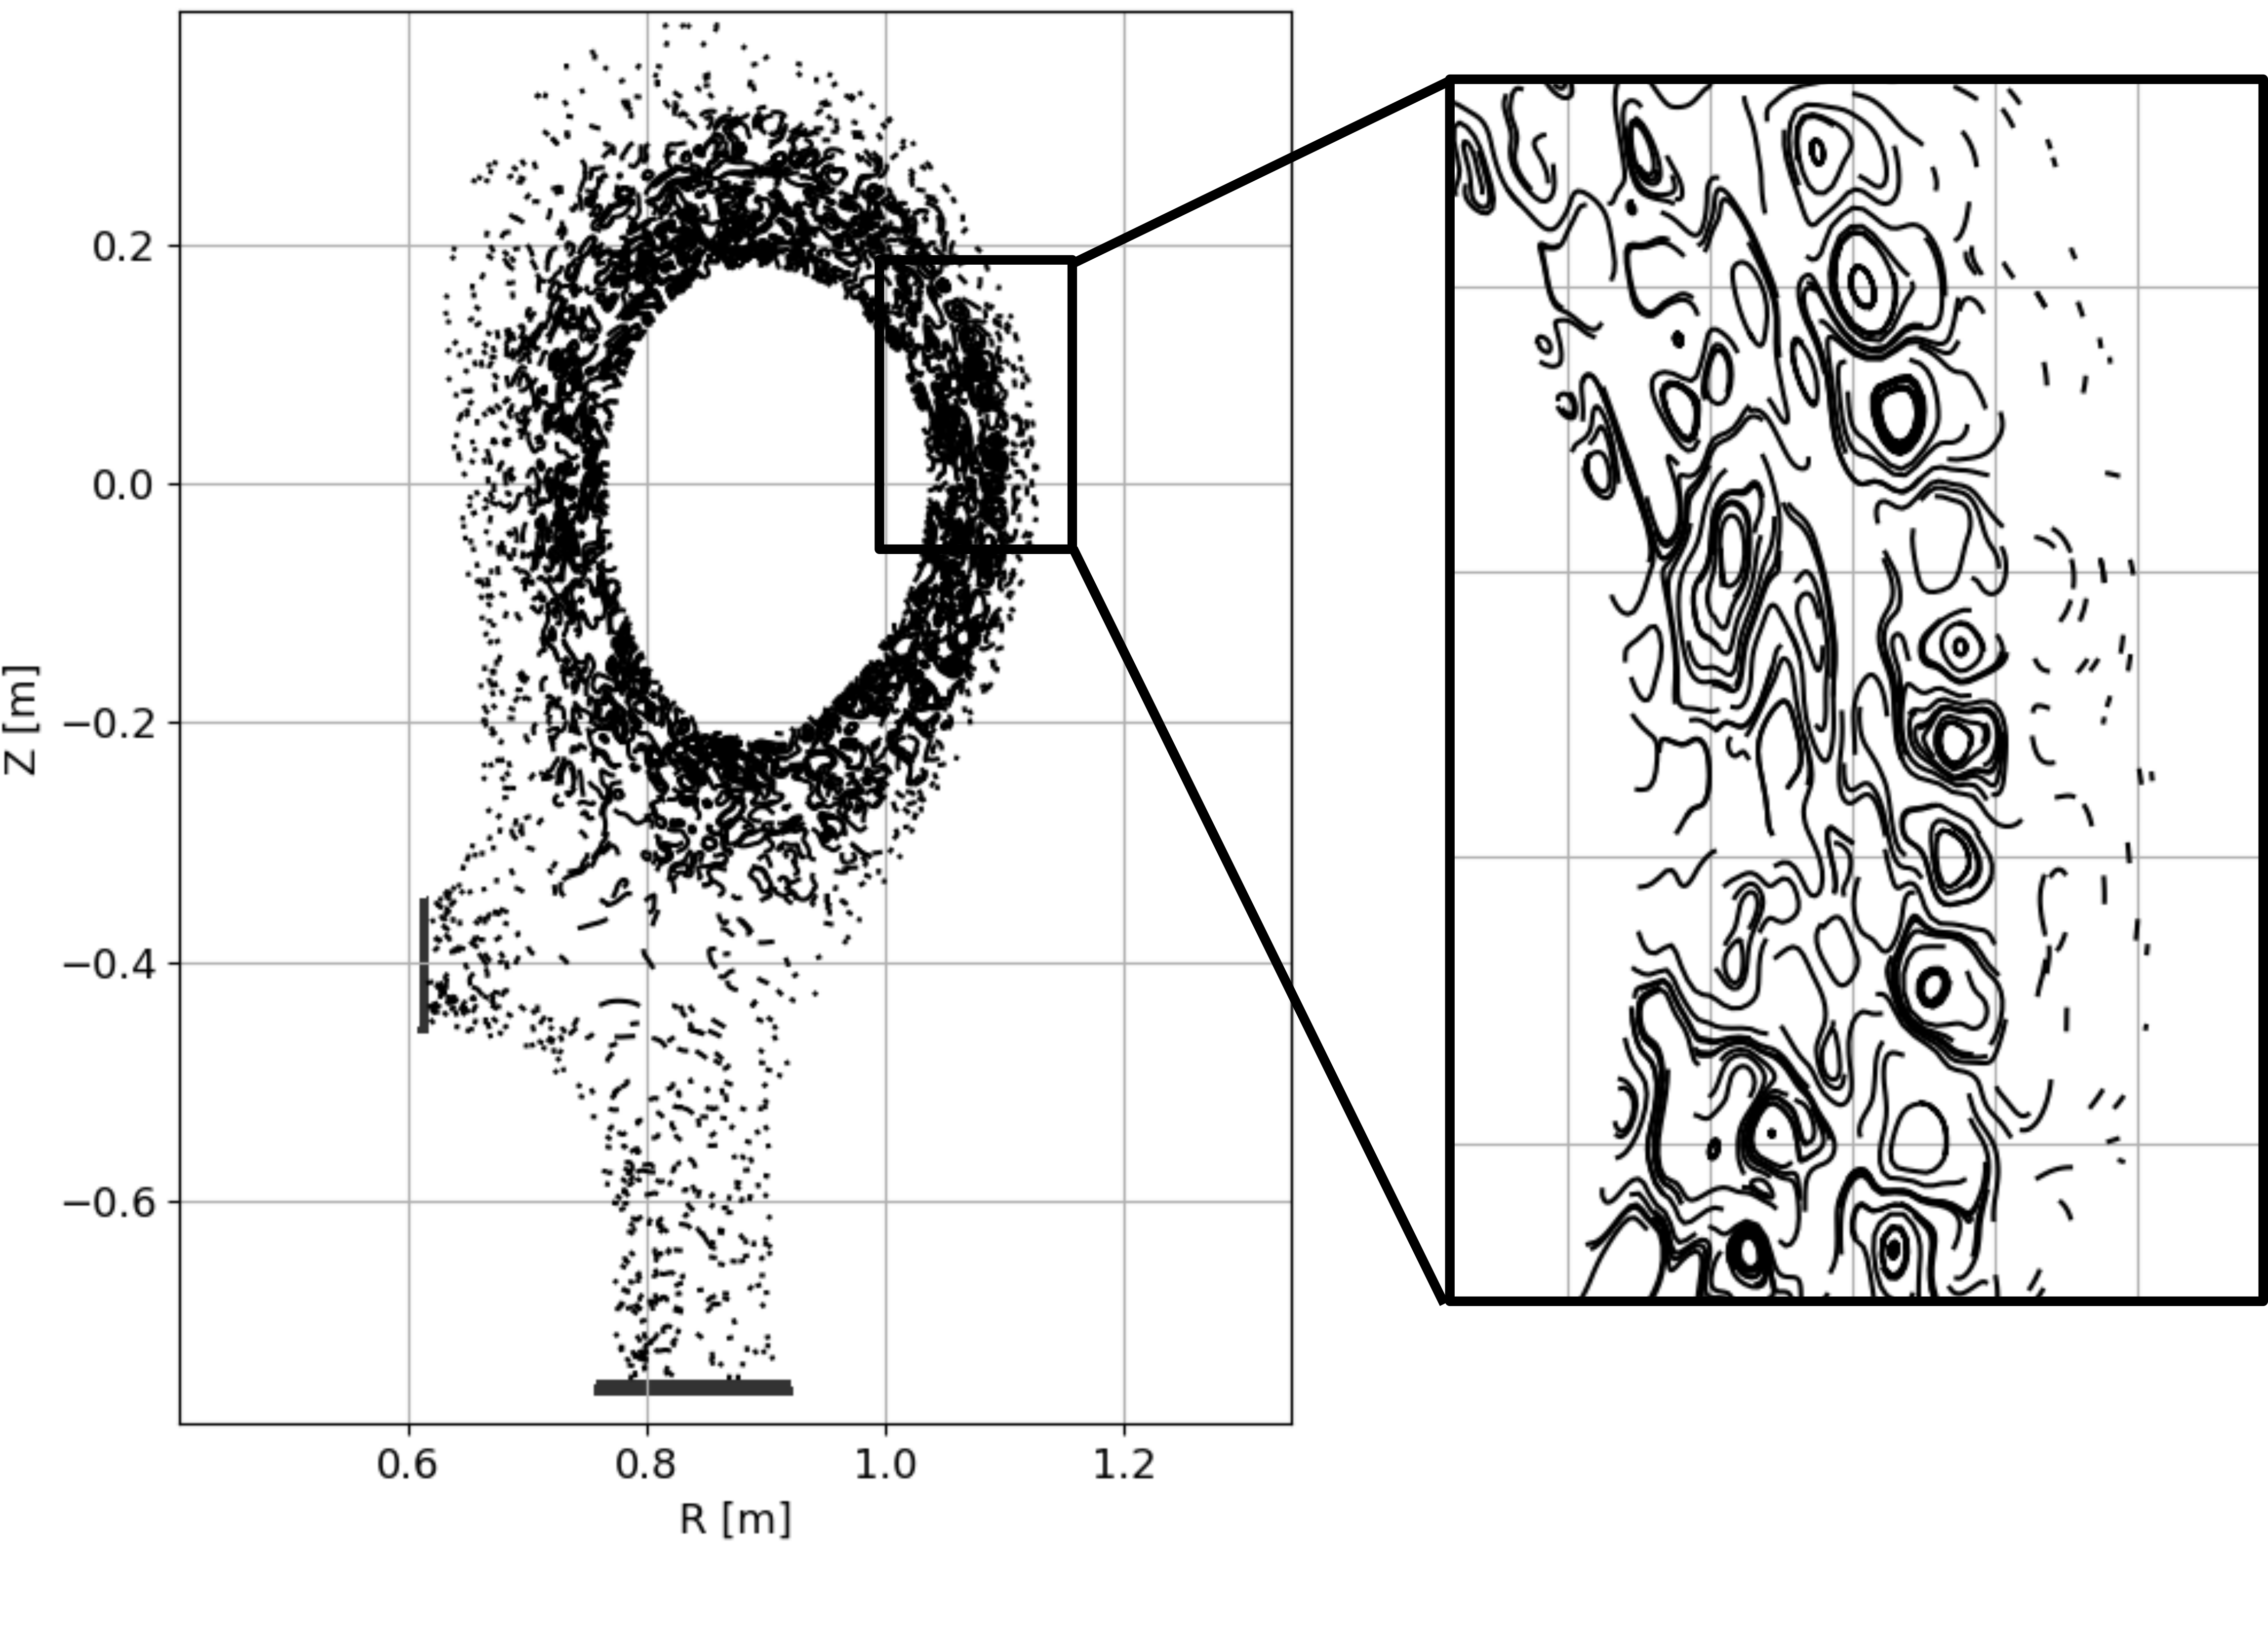
\includegraphics[width=1\textwidth]{schemes/poincareFlutterHighPower.png}
	\caption[Poincaré plot of the fluctuating magnetic field in the TCV high-power case for a random seed of 2500 points in a TCV poloidal plane]{Poincaré plot of the fluctuating magnetic field in the TCV high-power case for a random seed of 2500 points in a TCV poloidal plane.}
	\label{fig:TCV_poincareFlutter}	
\end{figure}

We observe the formation of islands whose centers are aligned with the separatrix. Their size corresponds approximately to typical turbulent filaments and their radial extent correlates to the region with steep temperature gradients. Some islands form also in vicinity to the core boundary, but this region is prone to artificial turbulence from the close heat source and fluid models  only have a limited validity there. A similar plot for the X21 flutter case, in App. \ref{sec:turbulentProfiles_poincareLmode}, does not exhibit any coherent structures, reinforcing the idea that the magnetic fluctuations play an important role for the transport barrier at high power. The exact physical mechanisms behind this observation still need to be investigated thoroughly.


\subsubsection{Grad-Shafranov shift}

In Sec. \ref{ssec:S3X_flutter}, we discussed the necessity of removing the equilibrium component from $A_\parallel$ before calculating the flutter field components. The concern was that $A_\parallel$ contains contributions from the Pfirsch-Schlüter current, which have already been accounted for in the poloidal flux function $\Psi$ that defines the equilibrium field $B_{pol}$. For the time being, we remove the toroidal average of $A_\parallel$ at each timestep, yielding stable simulations. The effects of this procedure are shown in Fig. \ref{fig:TCV_poloidalFieldGS}, where we compare the flutter field to $B_{pol}$ with and without removing the average. When the full $A_\parallel$ is used, large structures appear, particularly on the low-field side, reaching 13\% of the amplitude of $B_{pol}$. However, when we use only the toroidal fluctuations of $A_\parallel$ for the flutter, these structures disappear, leaving fine filaments at a much lower amplitude against a $\tilde{\textbf{B}}=0$ background. Thus, this pre-processing step for $A_\parallel$ appears necessary and effective. It also suggests that for the current applications of SOLEDGE3X, there is no need to apply an additional time-averaging process, as proposed by \cite{zhang2024}, since we do not observe transient structures.

\begin{figure}[H]\centering
	\begin{subfigure}[t]{0.3\textwidth}
		\centering
		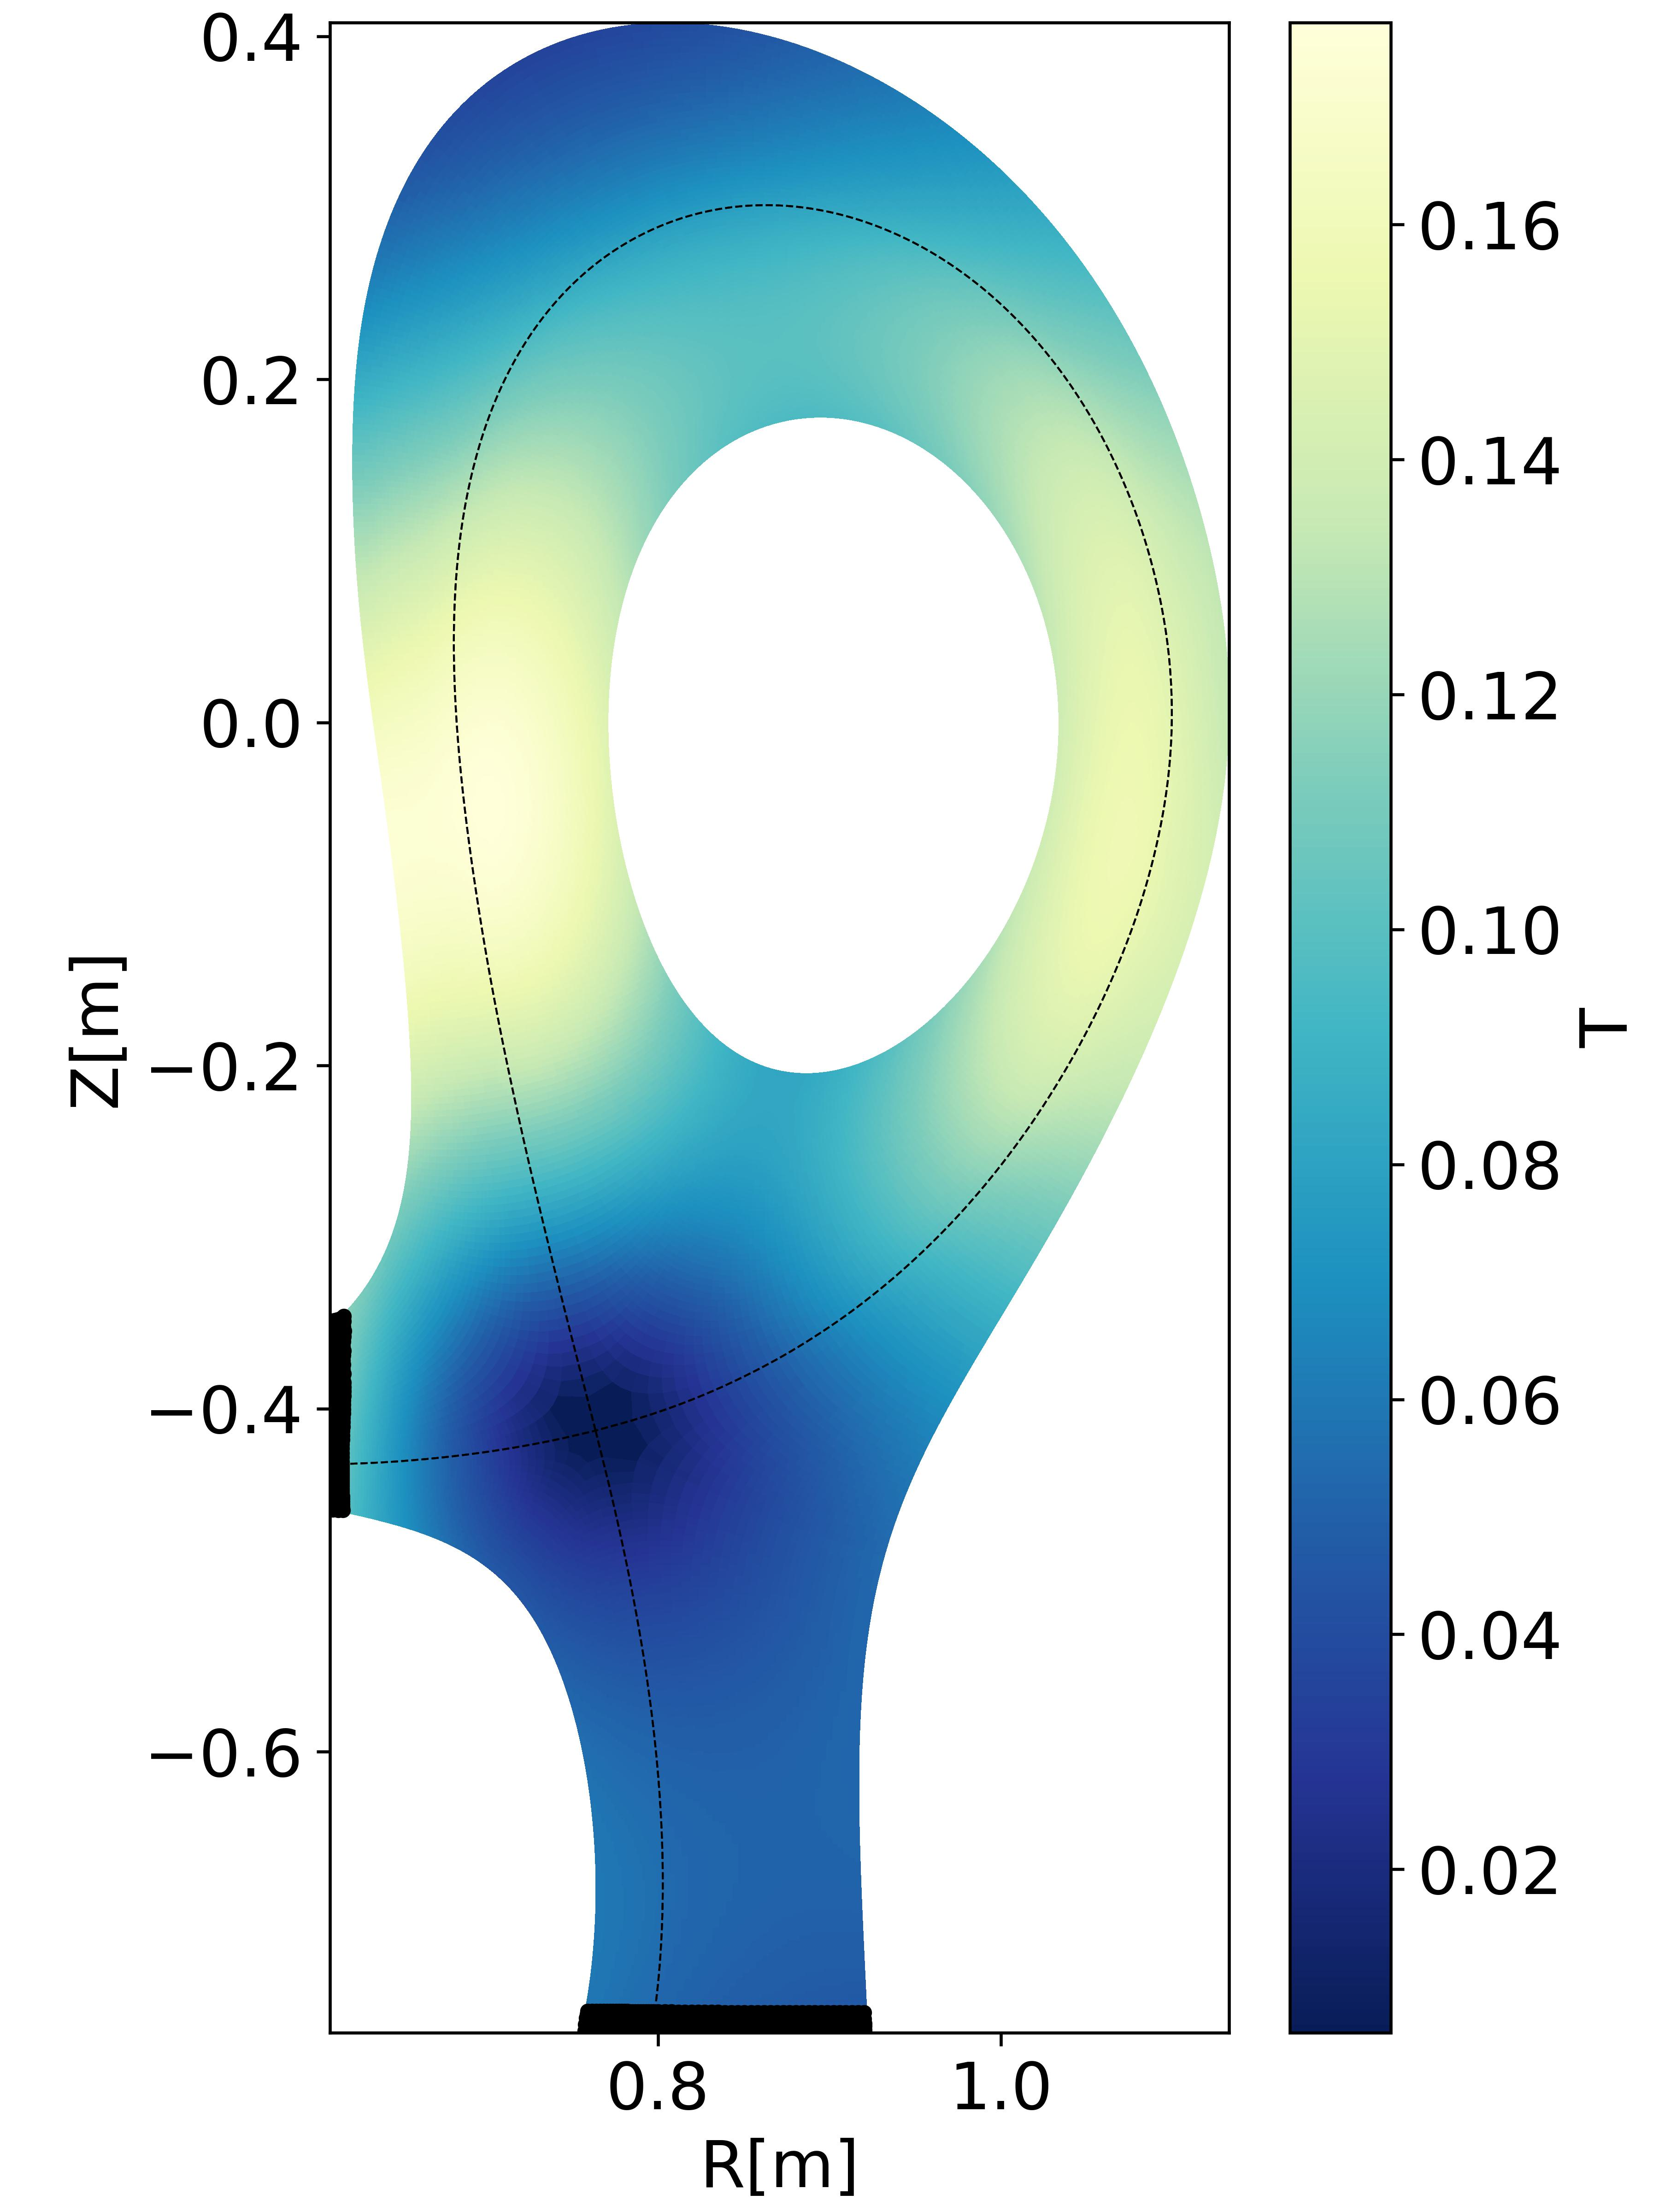
\includegraphics[width=1\textwidth]{schemes/Hmode_Bpol_eq.jpg}
		\subcaption{Equilibrium poloidal field}
		\label{fig:TCV_poloidalFieldGS_Beq}
	\end{subfigure}
	\begin{subfigure}[t]{0.3\textwidth}
		\centering
		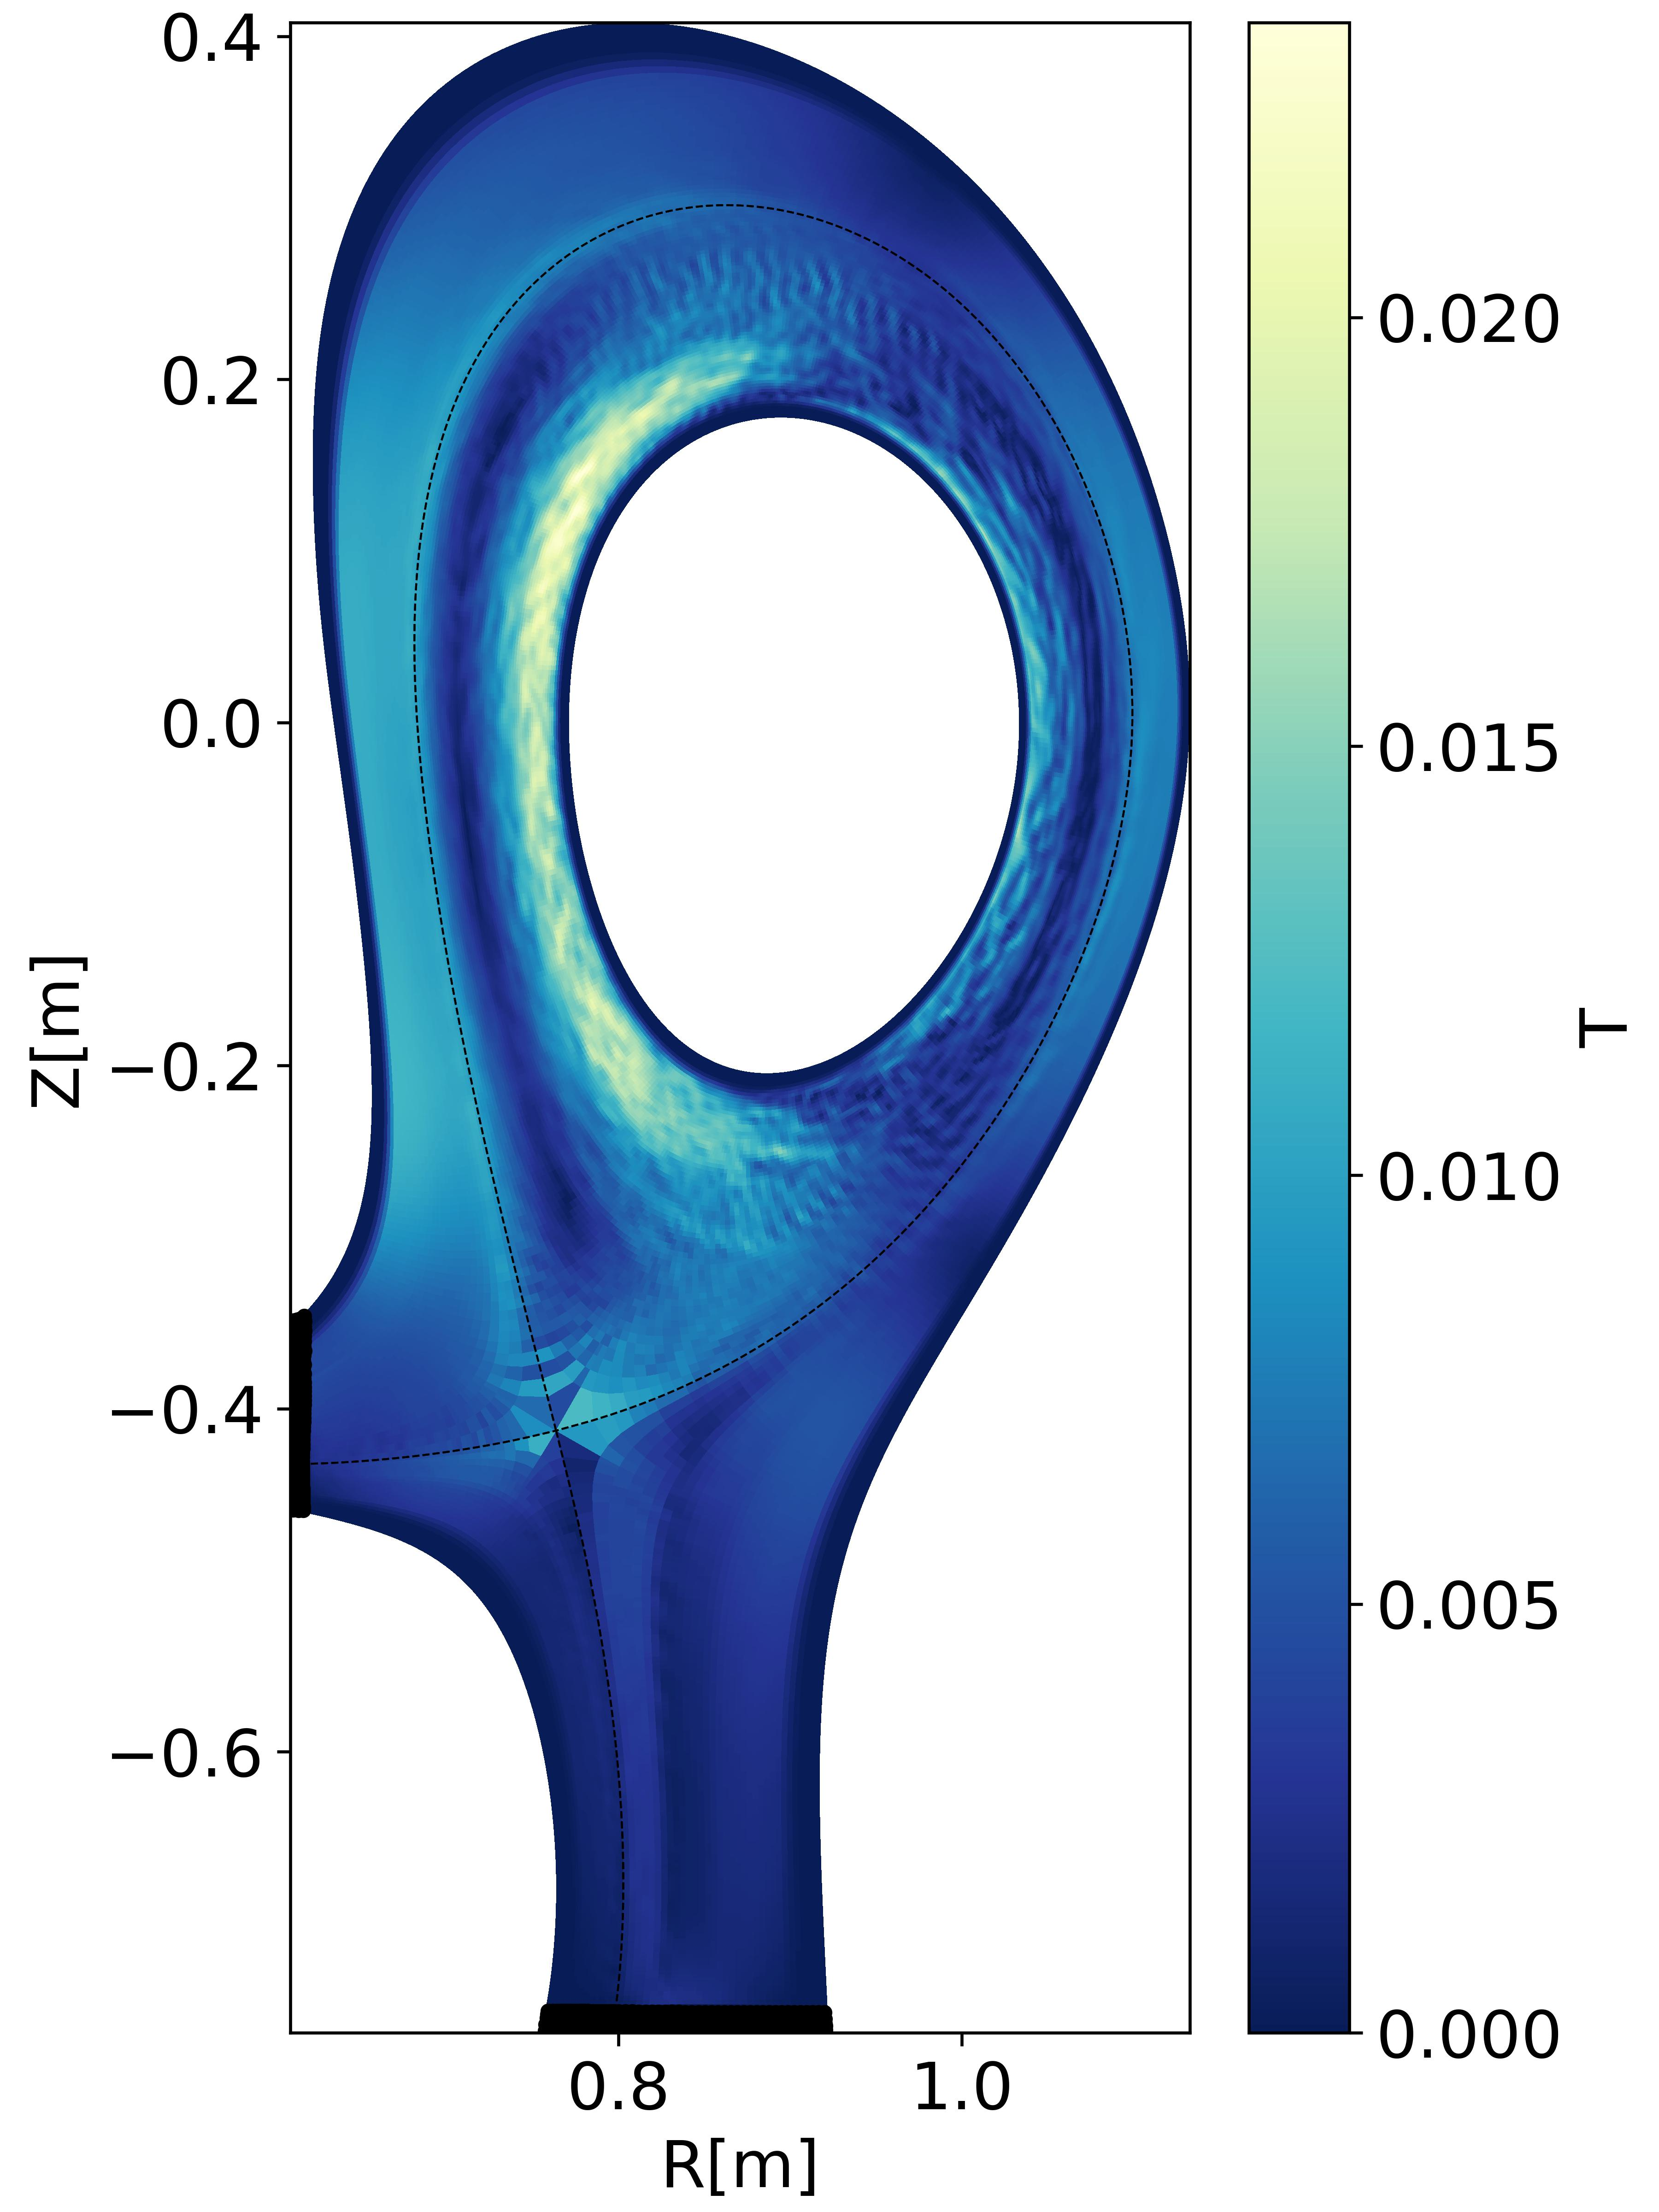
\includegraphics[width=1\textwidth]{schemes/Hmode_BEM_noAverage.jpg}
		\subcaption{Flutter field from \\ the full $A_\parallel$}
		\label{fig:TCV_poloidalFieldGS_Btilde_fullA}
	\end{subfigure}
	\begin{subfigure}[t]{0.3\textwidth}
		\centering
		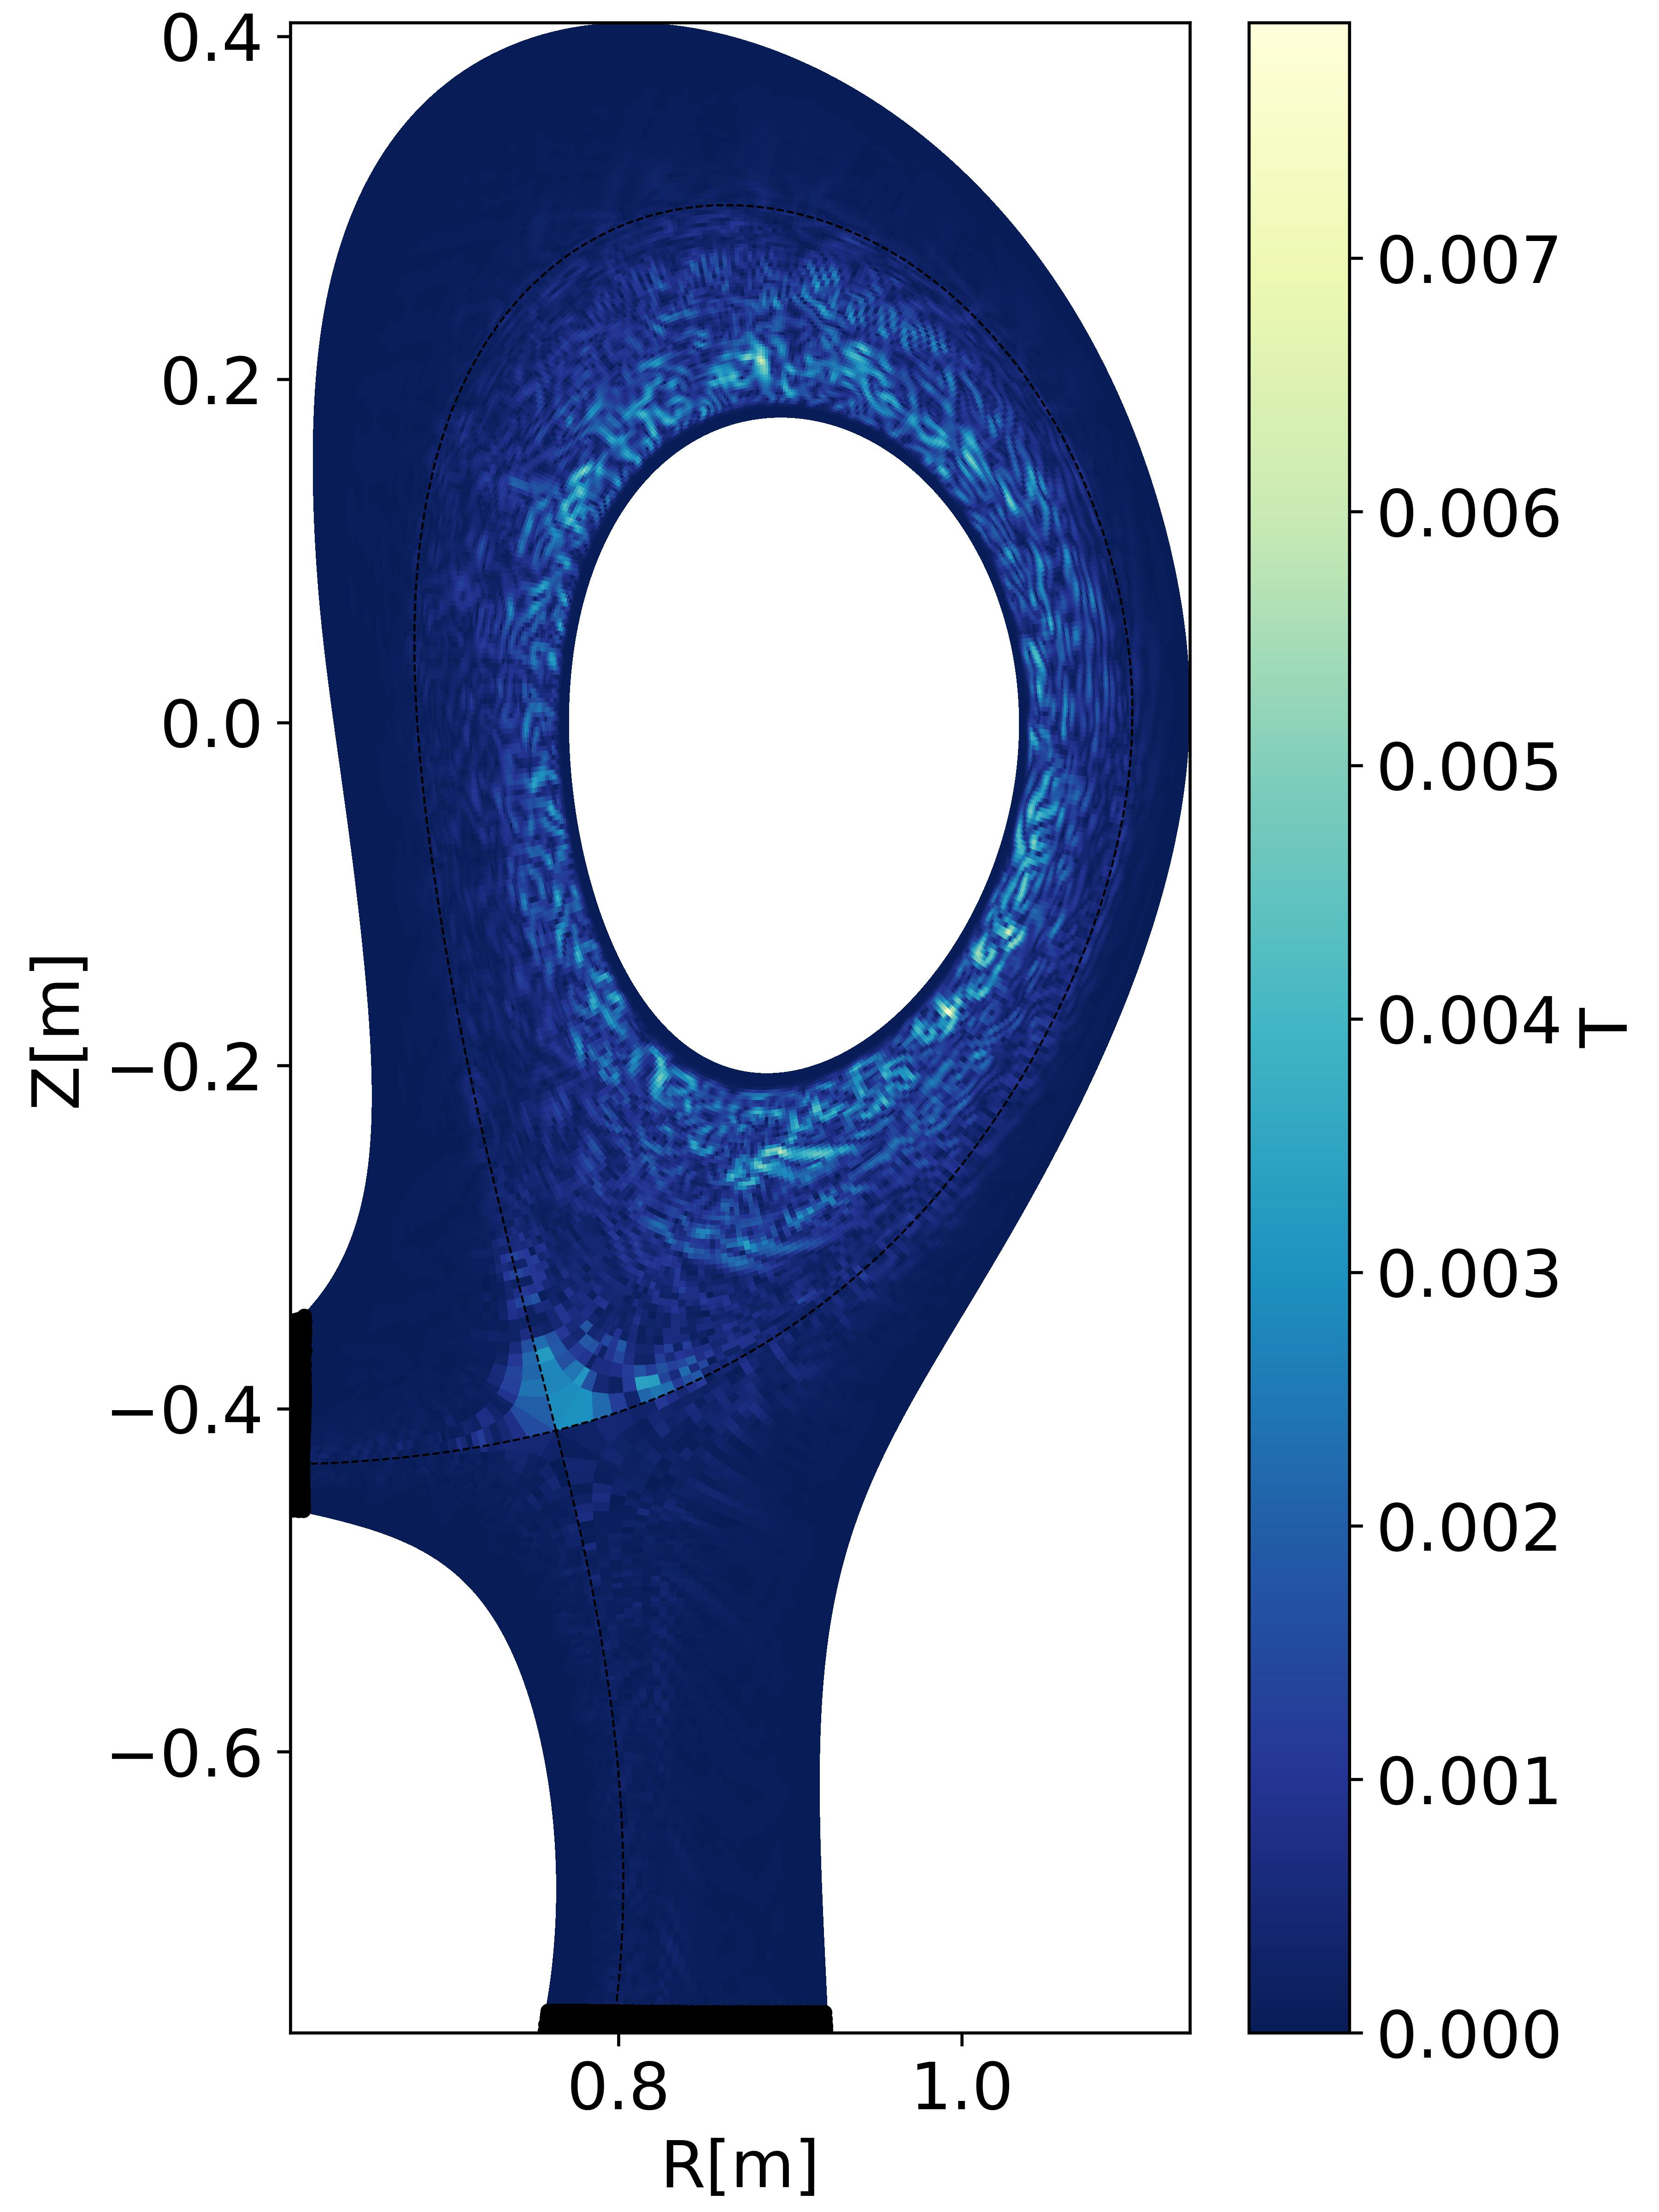
\includegraphics[width=1\textwidth]{schemes/Hmode_BEM_averaged.jpg}
		\subcaption{Flutter field from \\ the fluctuating $A_\parallel$}
		\label{fig:TCV_poloidalFieldGS_Btilde_fluctuatingA}
	\end{subfigure}
	\caption[Comparison of the magnitude of the flutter field to the poloidal magnetic field strength $B_{pol}$]{Comparison of the magnitude of the flutter field to the poloidal magnetic field strength $B_{pol}$. Snapshot on the first poloidal plane at the end of the high-power scenario.}
	\label{fig:TCV_poloidalFieldGS}
\end{figure}



%\section{Electromagnetic power scan}
%
%Full model, with electron inertia, magnetic induction and flutter. 
%
%Increase input power of the Ohmic heating in the TCV scenarios. Density is controlled by Horsten neutral model.
%
%\subsection{Qualitative evolution of the simulation}
%
%First phase the plasma heats up. As it reaches a quasi-steady state (surge in output heat fluxes to compensate the core source), Increase in turbulent transport across separatrix. But importantly: strong increase of the radial flutter flux.
%
%\subsection{Mid-plane profiles}
%
%
%\begin{figure}[H]\centering
%	\begin{subfigure}[t]{0.30\textwidth}
%		\centering
%		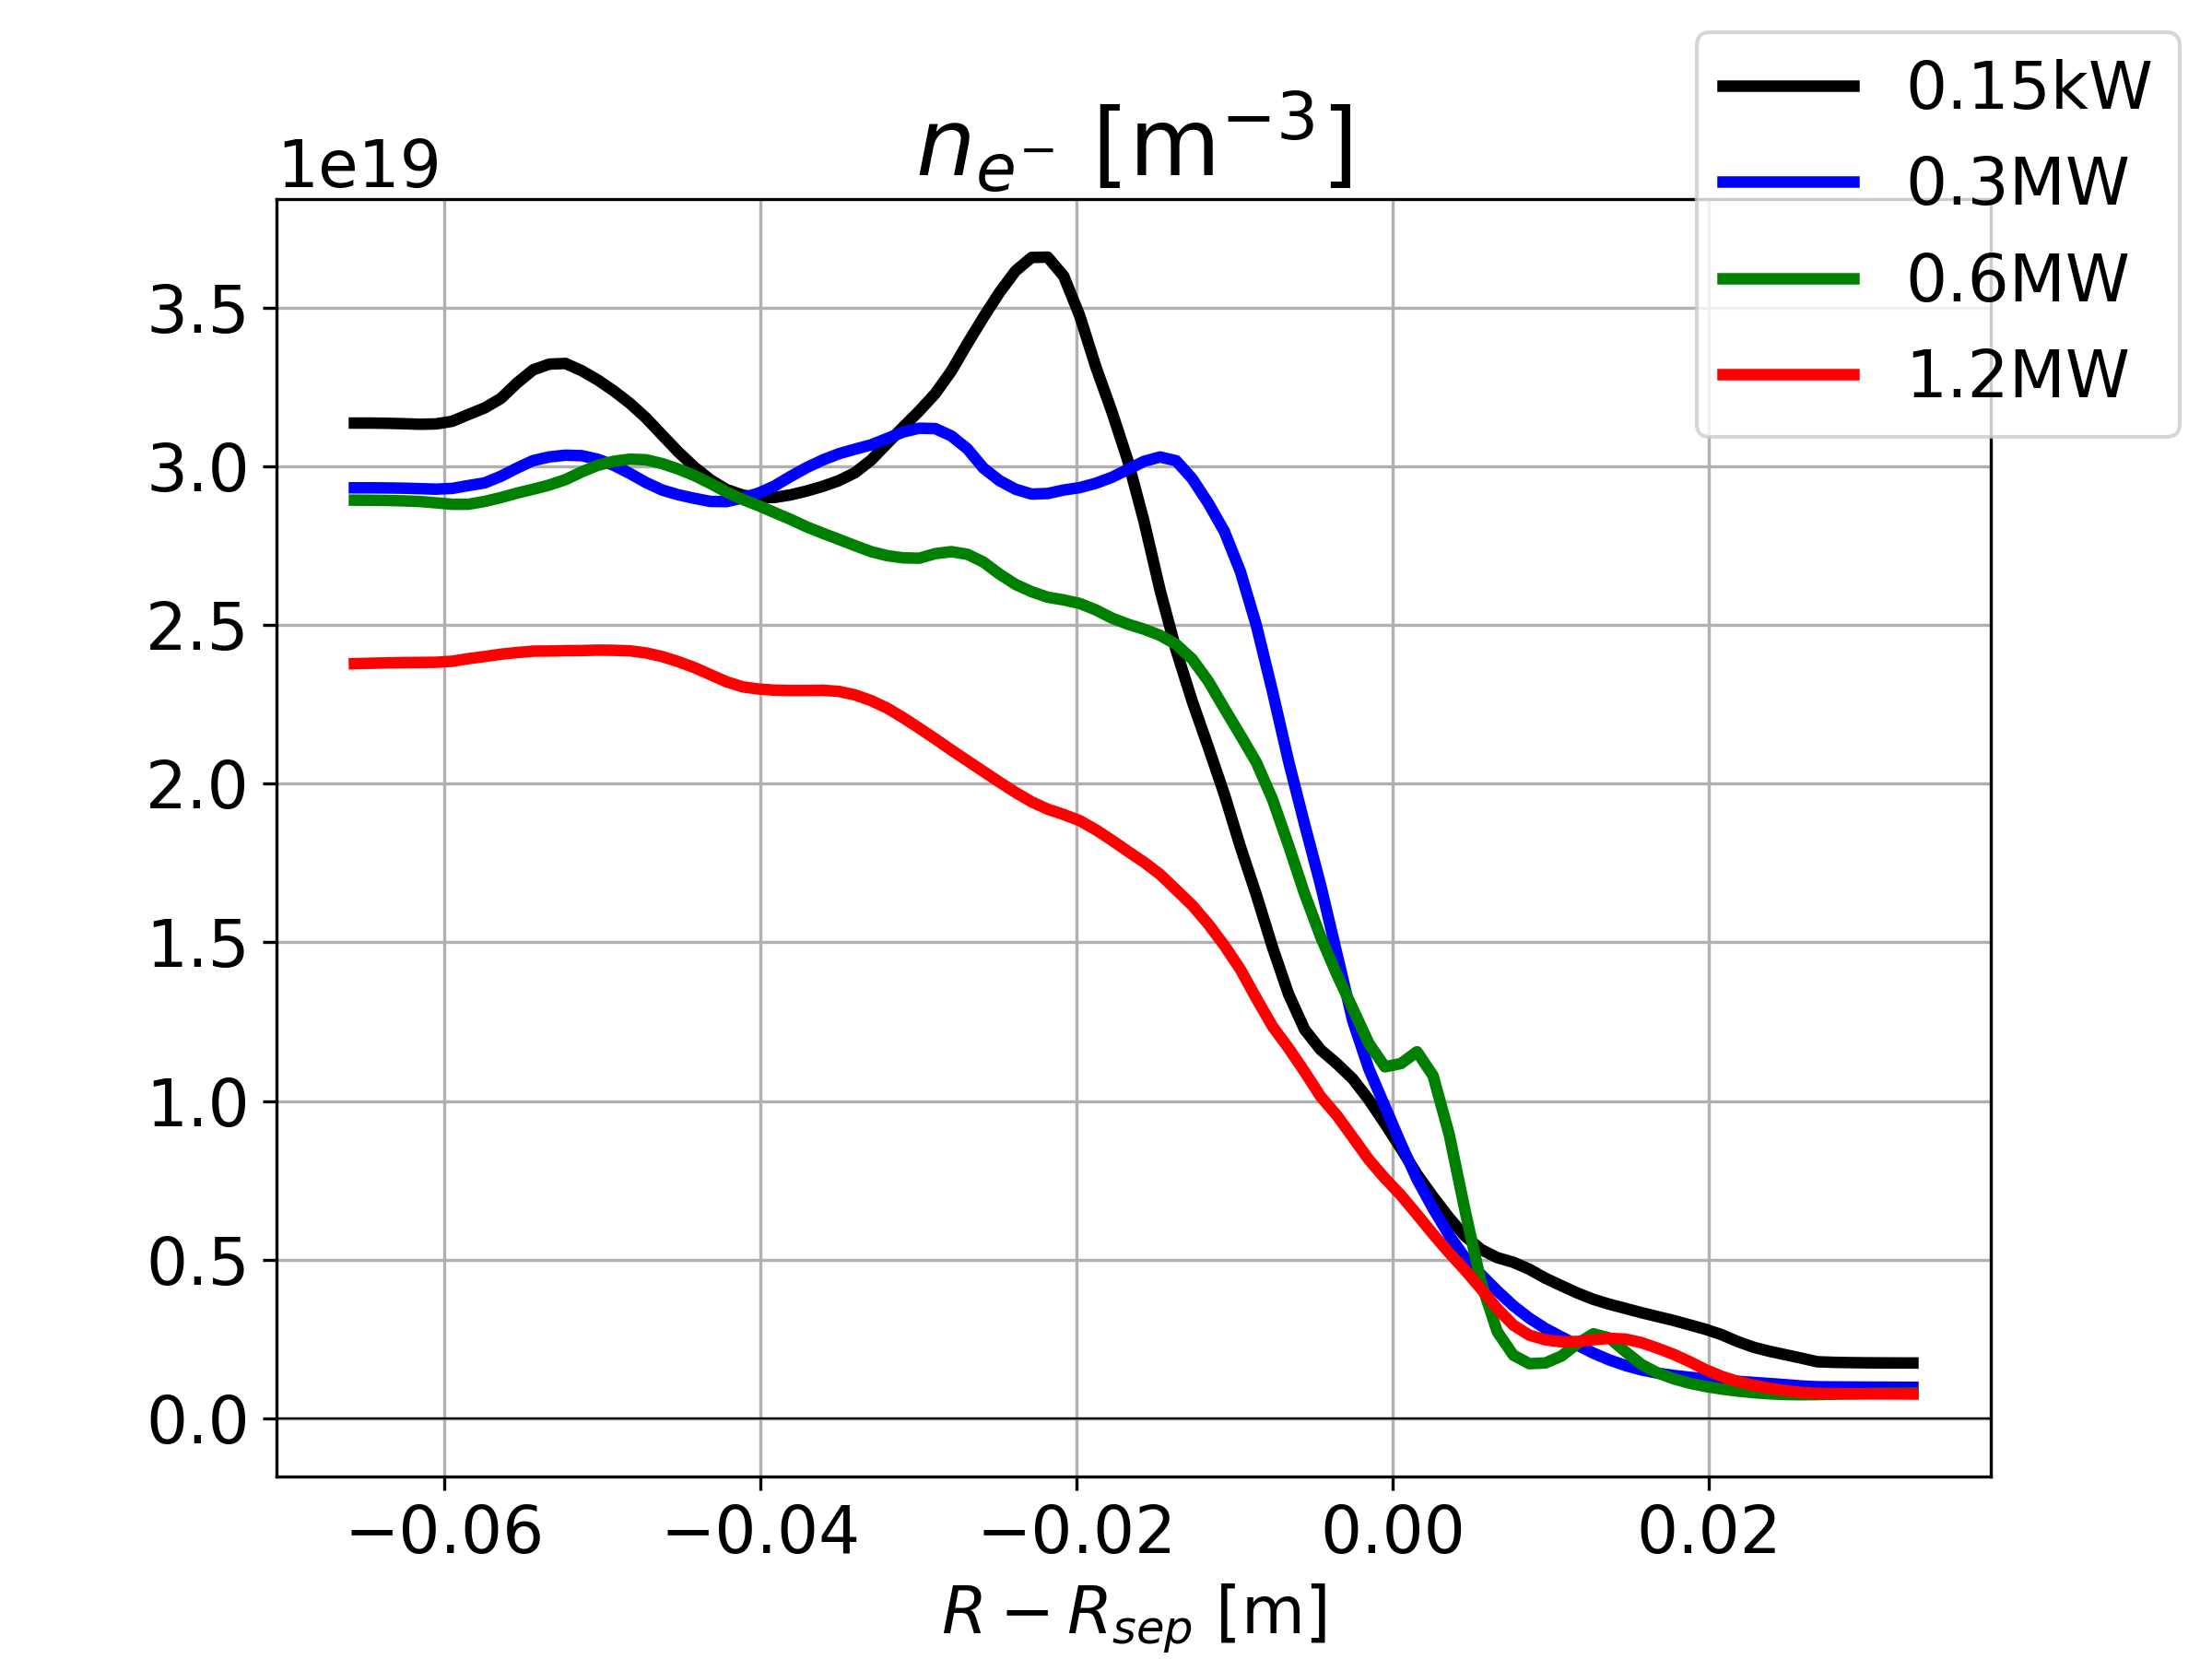
\includegraphics[width=1\textwidth]{schemes/TCVpowerScan_OMP_profiles_e-_n.png}
%		\subcaption{Plasma density $n$}
%	\end{subfigure}
%	\begin{subfigure}[t]{0.30\textwidth}
%		\centering
%		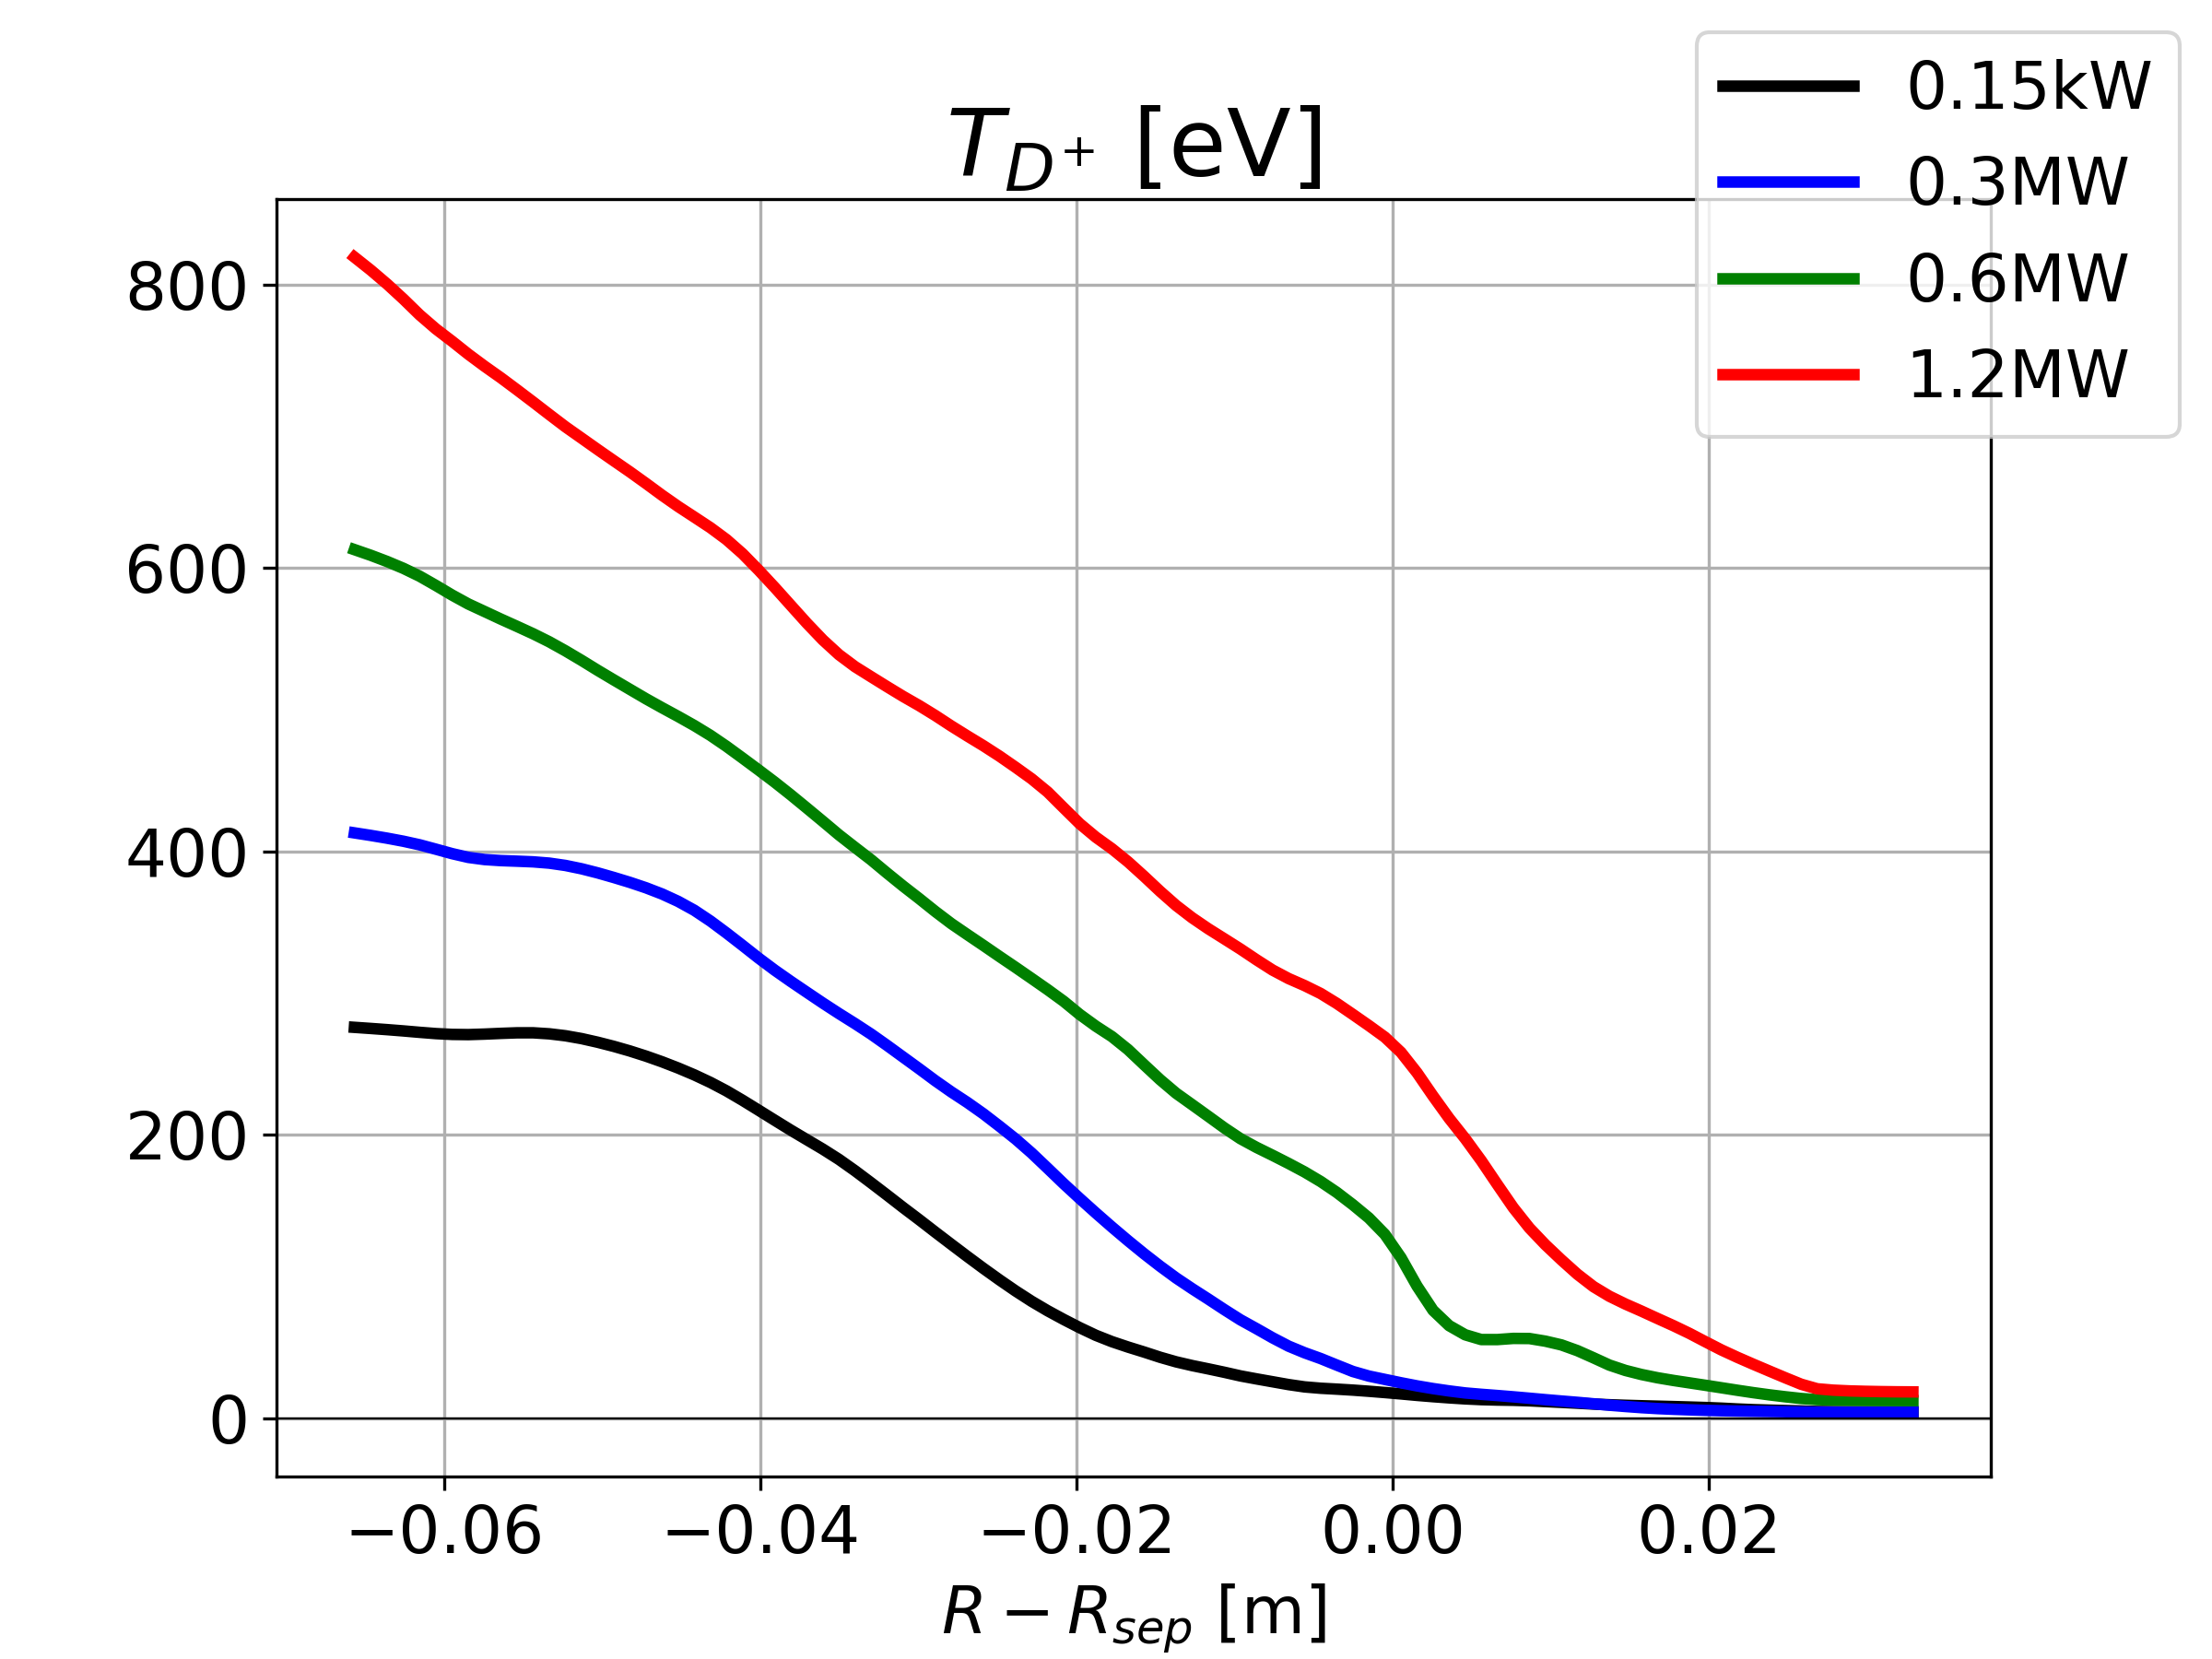
\includegraphics[width=1\textwidth]{schemes/TCVpowerScan_OMP_profiles_D+_T.png}
%		\subcaption{Electron temperature $T_e$}
%	\end{subfigure}
%	\begin{subfigure}[t]{0.30\textwidth}
%		\centering
%		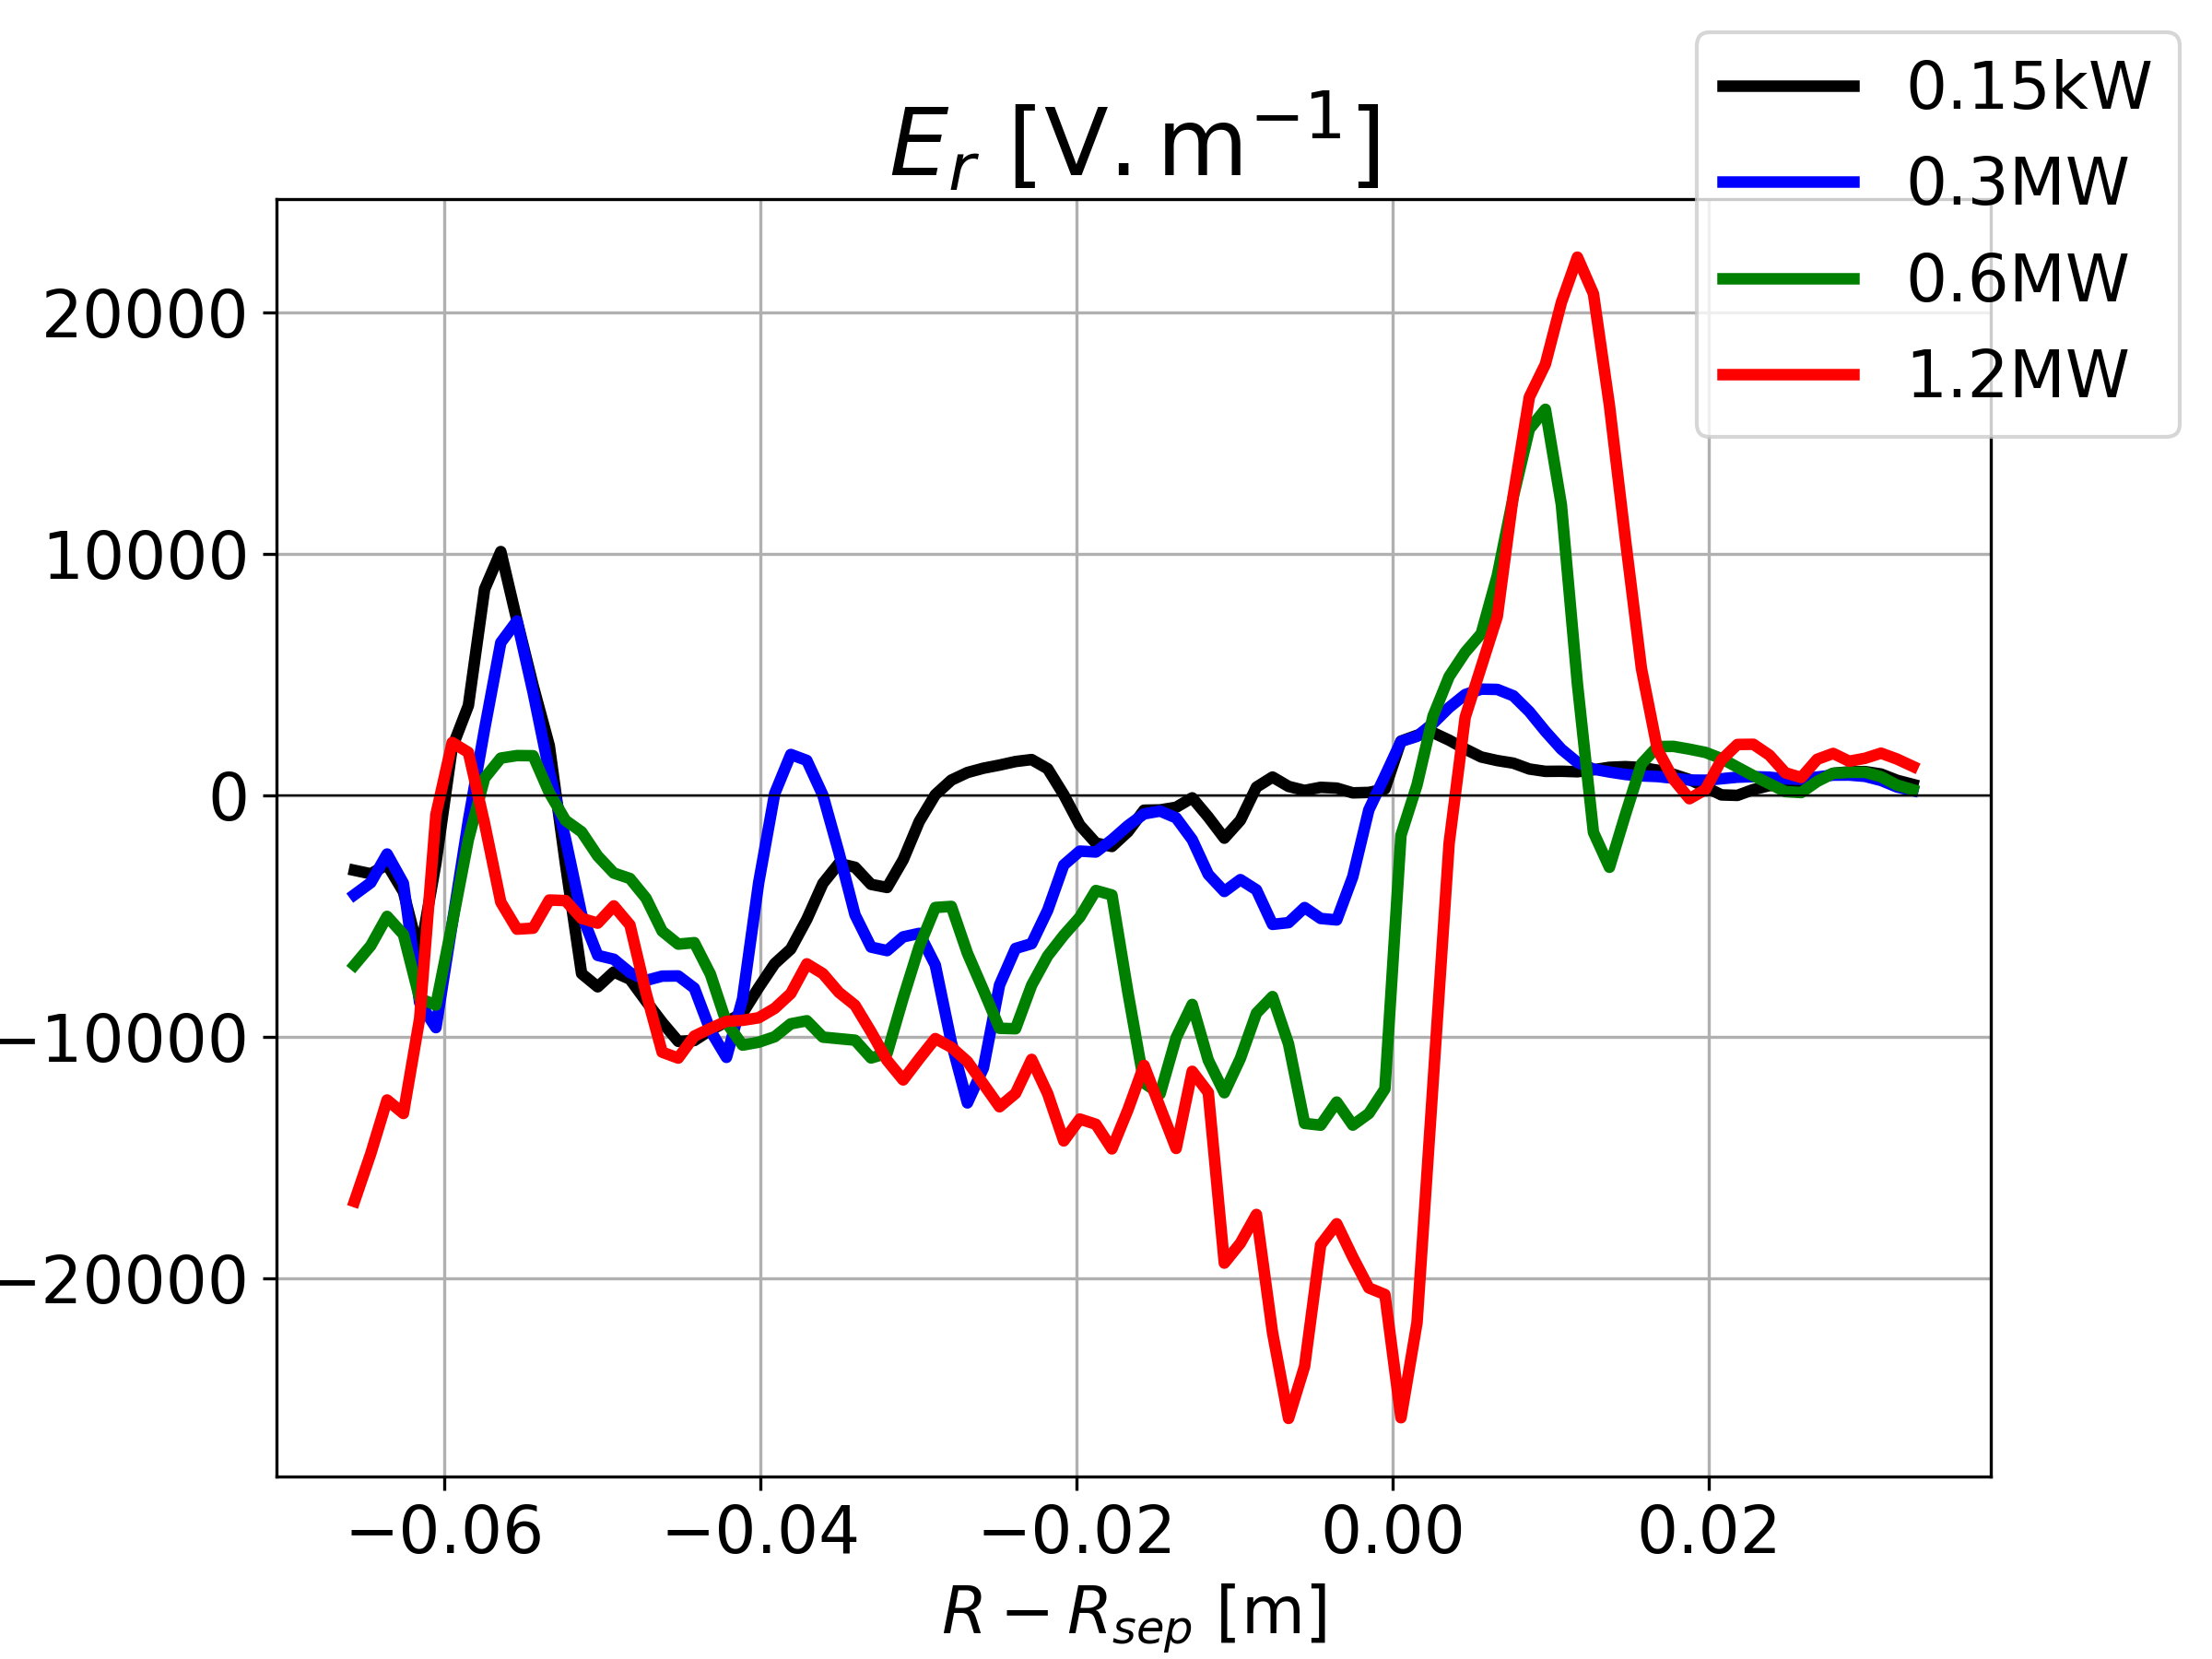
\includegraphics[width=1\textwidth]{schemes/TCVpowerScan_OMP_profiles_global_fields_E_r.png}
%		\subcaption{Electric potential $\Phi$}
%	\end{subfigure}
%	\caption{Radial profiles at the outer mid-plane after 4ms.}
%	\label{fig:TCV_powerScan_OMP_profiles}
%\end{figure}
%
%
%Formation of a pedestal ?
%
%









